\documentclass{beamer}


%%%%% 26-02-2022 package multicol multirow
\newcommand{\mc}[2]{\multicolumn{#1}{c}{#2}}
\definecolor{Gray}{gray}{0.85}
\definecolor{LightCyan}{rgb}{0.88,1,1}
\usepackage{hhline,longtable}
\usepackage{tabularx,booktabs}

\usepackage{multicol}
\usepackage{multirow}
%% 26-02-2022
\usepackage{hhline,longtable}
\usepackage{threeparttable}

\usepackage{tabularx,booktabs}
\newcommand{\tabitem}{~~\llap{\textbullet}~~}


\usepackage{enumerate}
\usepackage[shortlabels]{enumitem}

\setlist[enumerate, 1]{label =\textbf{\arabic*.}}
\setlist[enumerate, 2]{label =\textbf{\theenumi \alph*}}
\usepackage{array,multirow}

\usepackage{amsmath,mathtools}

\usepackage{amssymb}
\usepackage{amsthm}
\usepackage{mathtools}



\DeclarePairedDelimiter\abs{\lvert}{\rvert}%
\DeclarePairedDelimiter\norm{\lVert}{\rVert}%

% Swap the definition of \abs* and \norm*, so that \abs
% and \norm resizes the size of the brackets, and the 
% starred version does not.
\makeatletter
\let\oldabs\abs
\def\abs{\@ifstar{\oldabs}{\oldabs*}}










%%%% animation package 21-09-2021
\usepackage{animate}


%%%%%%%%%%%%%%%%%09-09-2021\\\ copied from Webinarinnovation page
% Here I would like to make a new command to change the transparency of a photo and put it as a background photo
\usepackage{tikz}



%%%%%%%%%%%% 22-10-2020 Background block package
% beamer: How to place images behind text (z-order)
% (http://tex.stackexchange.com/a/134311)
\makeatletter
\newbox\@backgroundblock
\newenvironment{backgroundblock}[2]{%
  \global\setbox\@backgroundblock=\vbox\bgroup%
    \unvbox\@backgroundblock%
    \vbox to0pt\bgroup\vskip#2\hbox to0pt\bgroup\hskip#1\relax%
}{\egroup\egroup\egroup}
\addtobeamertemplate{background}{\box\@backgroundblock}{}
\makeatother

%%%%%%%%%%%%%%%%%%%%%%%%%%%%%%%%%%%%%%%%%%%%
%%%%%%%%%%%26-10-2020% set figure number
\setbeamertemplate{caption}[numbered]


%%%%%%%%%%%%%%%%26-10-2020
\usepackage{amssymb,amsmath}


%%%%%%%%%%%%%%%%26-10-2020
\newenvironment{variableblock}[3]{%
  \setbeamercolor{block body}{#2}
  \setbeamercolor{block title}{#3}
  \begin{block}{#1}}{\end{block}}
  
  \setbeamercolor{block body alerted}{bg=alerted text.fg!10}
\setbeamercolor{block title alerted}{bg=alerted text.fg!20}
\setbeamercolor{block body}{bg=structure!10}
\setbeamercolor{block title}{bg=structure!20}
\setbeamercolor{block body example}{bg=green!10}
\setbeamercolor{block title example}{bg=green!20}

\setbeamertemplate{blocks}[rounded][shadow=true]


%%%%%%%%%%%%%%%%%%%%%26-10-2020
\setbeamertemplate{footline}[frame number]

%%%%%%%%%%%% 26-10-2020
\usepackage{color, colortbl}
\definecolor{Gray}{gray}{0.85}

%%%%%%%%%%%%%%%%%%27-10-2020
\usepackage[T1]{fontenc}



\title{\large \textbf{Large-Scale Integration of EVs, one Application of the High-Performace Solver: BATTPOWER}}
\begin{backgroundblock}{20mm}{20mm}
    \begin{tikzpicture}
    \node[anchor=east,inner sep=0] (B) at (4,0) {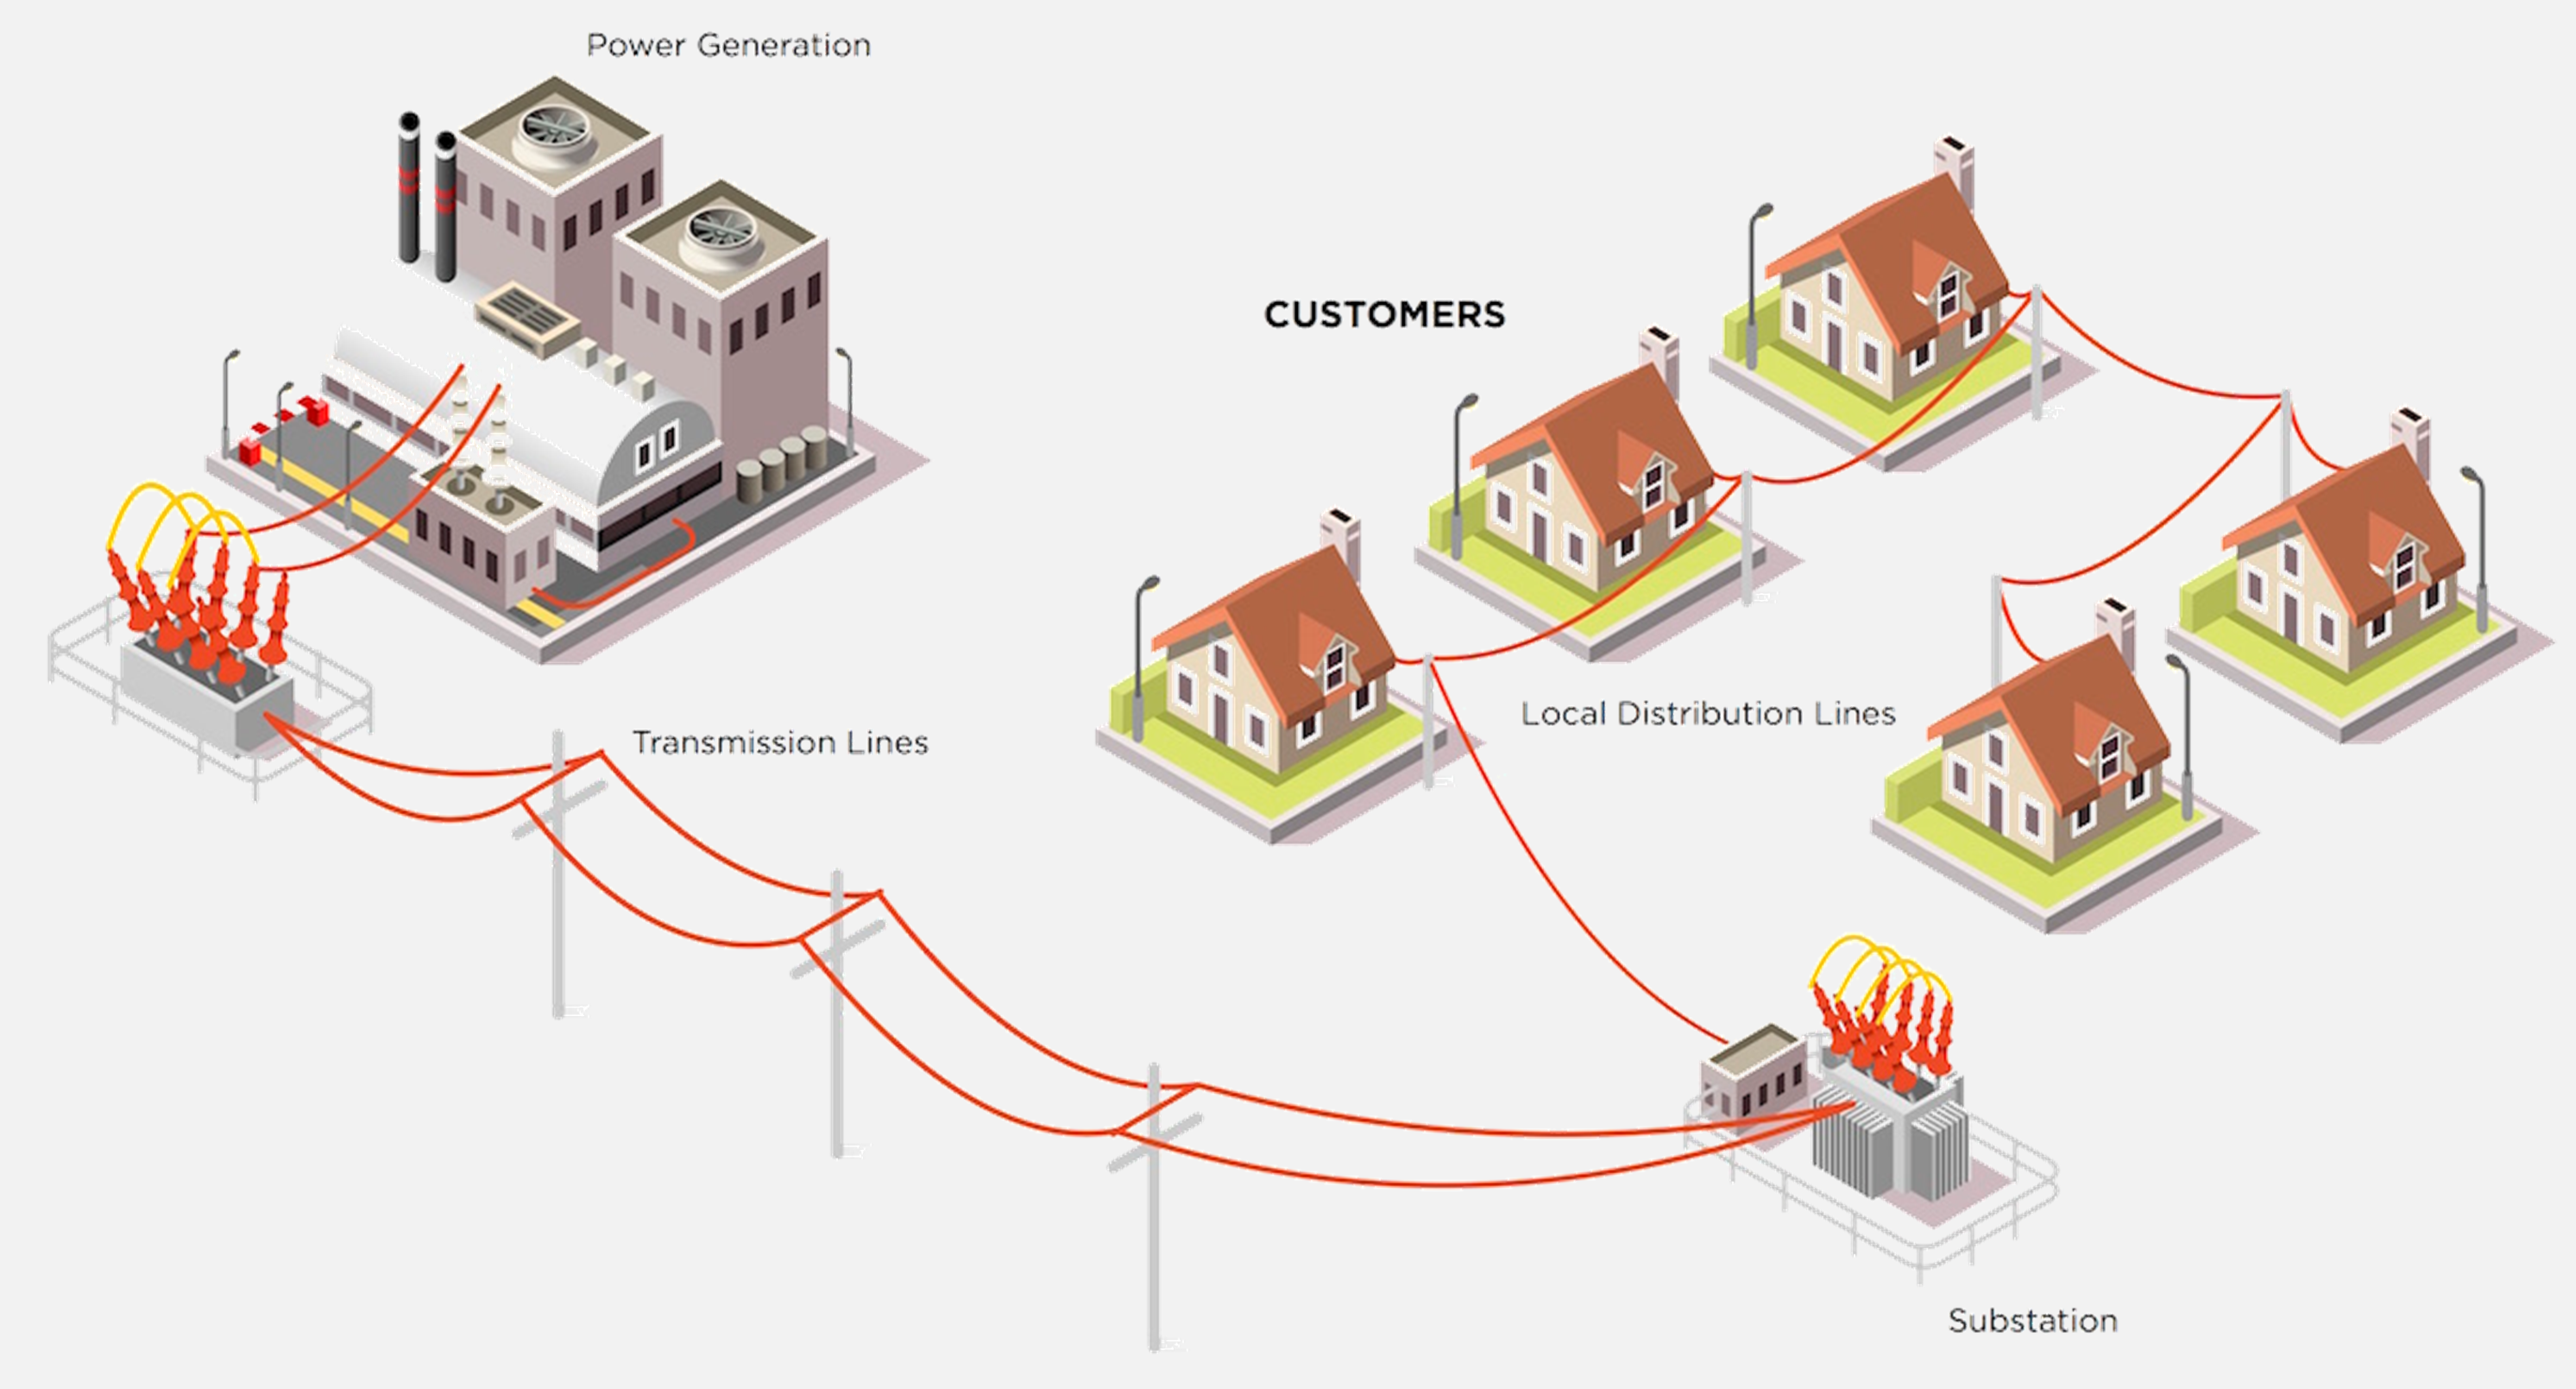
\includegraphics[width=\linewidth]{Figures/PowerSys.png}};
           \fill [draw=none, fill=white, fill opacity=0.7] (B.north west) -- (B.north east) -- (B.south east) -- (B.south west) -- (B.north west) -- cycle;
 
    \end{tikzpicture} 
    \end{backgroundblock} 

\logo{%
    
\includegraphics[width=3cm,height=3cm,keepaspectratio]{ntnulogo_eng}~%
}


\author{Salman Zaferanlouei}
\institute{NTNU{\\ \vskip 1cm} \scalebox{1.5}{\insertlogo}}
\date{\today}









\begin{document}
\begin{frame}
\titlepage
\end{frame}
%%%%%%%%%%%%%%%%%%%%%%%%%%%%%%%%%%%%%%%%%%
%%%%%%%%%%%%%%%%%%%%%%%%%%%%%%%%%%%%%%%%%%
%%%%%%%%%%%%%%%%%%%%%%%%%%%%%%%%%%%%%%%%%%
%%%%%%%%%%%%%%%%%%%%%%%%%%%%%%%%%%%%%%%%%%
%%%%%%%%%%%%%%%%%%%%%%%%%%%%%%%%%%%%%%%%%
%%%%%%%%%%%%%%%%%%%%%%%%%%%%%%%%%%%%%%%%%%
%%%%%%%%%%%%%%%%%%%%%%%%%%%%%%%%%%%%%%%%%%
%%%%%%%%%%%%%%%%%%%%%%%%%%%%%%%%%%%%%%%%%%





\section{Purpose/Content}
\begin{frame}{The presentation goal}
\begin{itemize}
\item \textbf{Purpose:} To discuss how to solve multi-period optimal power flow fast; \textcolor{red}{\textbf{Large-Scale simulation with respect to time and space.}}
\item \textbf{Phase I:} Background and Motivation
\item \textbf{Phase II:} Power Flow and Optimal Power Flow
\item \textbf{Phase III:} Solution Method
\item \textbf{Phase IV:} Speed up
\item \textbf{Phase V:} Future Work

\end{itemize}
\begin{center}
\begin{tabular}{|l l|} 
\hline
\textbf{Presentation Time:}& 15-20 min \\
\hline
\end{tabular}
\end{center}
\end{frame}
%%%%%%%%%%%%%%%%%%%%%%%%%%%%%%%%%%%%%%%%%%
%%%%%%%%%%%%%%%%%%%%%%%%%%%%%%%%%%%%%%%%%%


\begin{frame}[plain]
\begin{tikzpicture}[overlay, remember picture]
\node[anchor=center] at (current page.center) {
\begin{beamercolorbox}[center]{title}
     Phase I:\\\textbf{Background and Motivation}
  \end{beamercolorbox}};
\end{tikzpicture}

\end{frame}
%%%%%%%%%%%%%%%%%%%%%%%%%%%%%%%%%%%%%%%%%
%%%%%%%%%%%%%%%%%%%%%%%%%%%%%%%%%%%%%%%%%%
%%%%%%%%%%%%%%%%%%%%%%%%%%%%%%%%%%%%%%%%%%
%%%%%%%%%%%%%%%%%%%%%%%%%%%%%%%%%%%%%%%%%
%%%%%%%%%%%%%%%%%%%%%%%%%%%%%%%%%%%%%%%%%%
%%%%%%%%%%%%%%%%%%%%%%%%%%%%%%%%%%%%%%%%%%
%%%%%%%%%%%%%%%%%%%%%%%%%%%%%%%%%%%%%%%%%%
%%%%%%%%%%%%%%%%%%%%%%%%%%%%%%%%%%%%%%%%%%
\section{Background}
\begin{frame}{Electricity Grid}
\begin{figure}[!htbp]
\centering
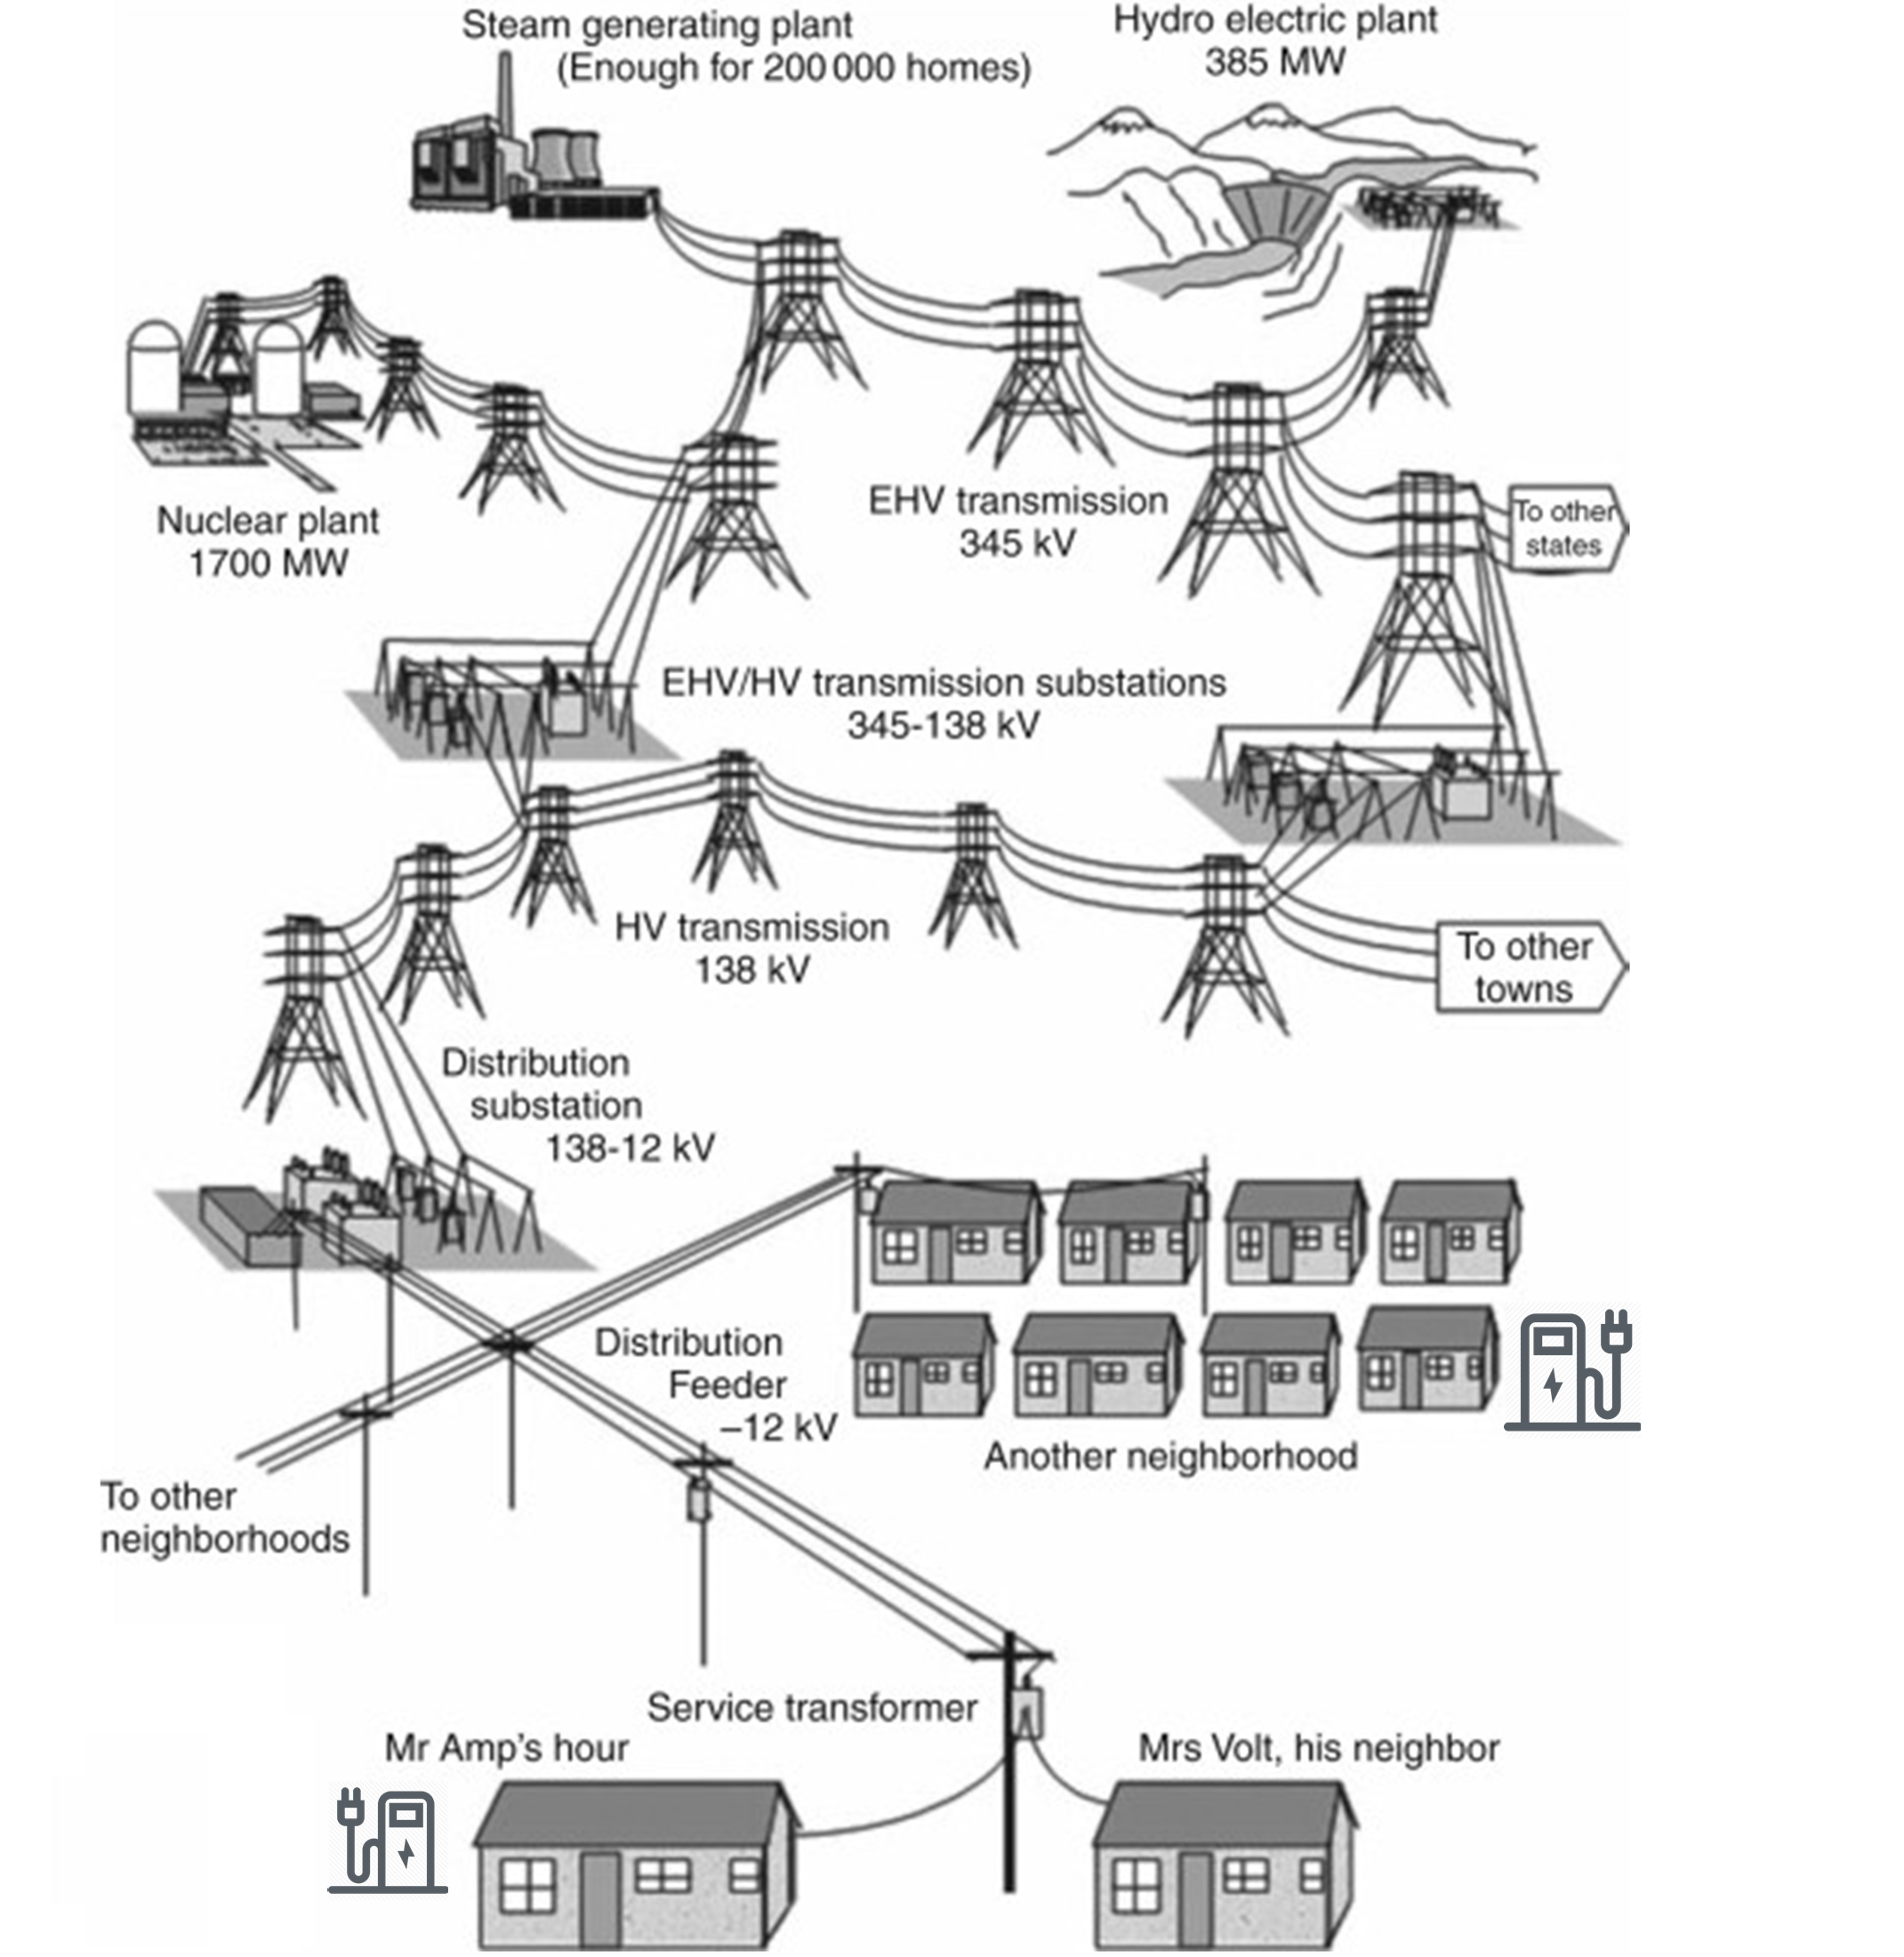
\includegraphics[width=2.8 in , height=2.4 in]{Figures/EVchalendge1.png}
\caption{\tiny[www.sciencedirect.com/science/article/pii/B9781845697846500019 ]}
\end{figure}
\end{frame}


%
%%%%%%%%%%%%%%%%%%%%%%%%%%%%%%%%%%%%%%%%%%
%%%%%%%%%%%%%%%%%%%%%%%%%%%%%%%%%%%%%
%%%%%%%%%%%%%%%%%%%%%%%%%%%%%%%%%%%%%%%%%%
%%%%%%%%%%%%%%%%%%%%%%%%%%%%%%%%%%%%%%%%%%
%%%%%%%%%%%%%%%%%%%%%%%%%%%%%%%%%%%%%%%%%%
%%%%%%%%%%%%%%%%%%%%%%%%%%%%%%%%%%%%%%%%%%
%\section{Background}
%\begin{frame}{Electricity Grid}
%\begin{figure}[!htbp]
%\centering
%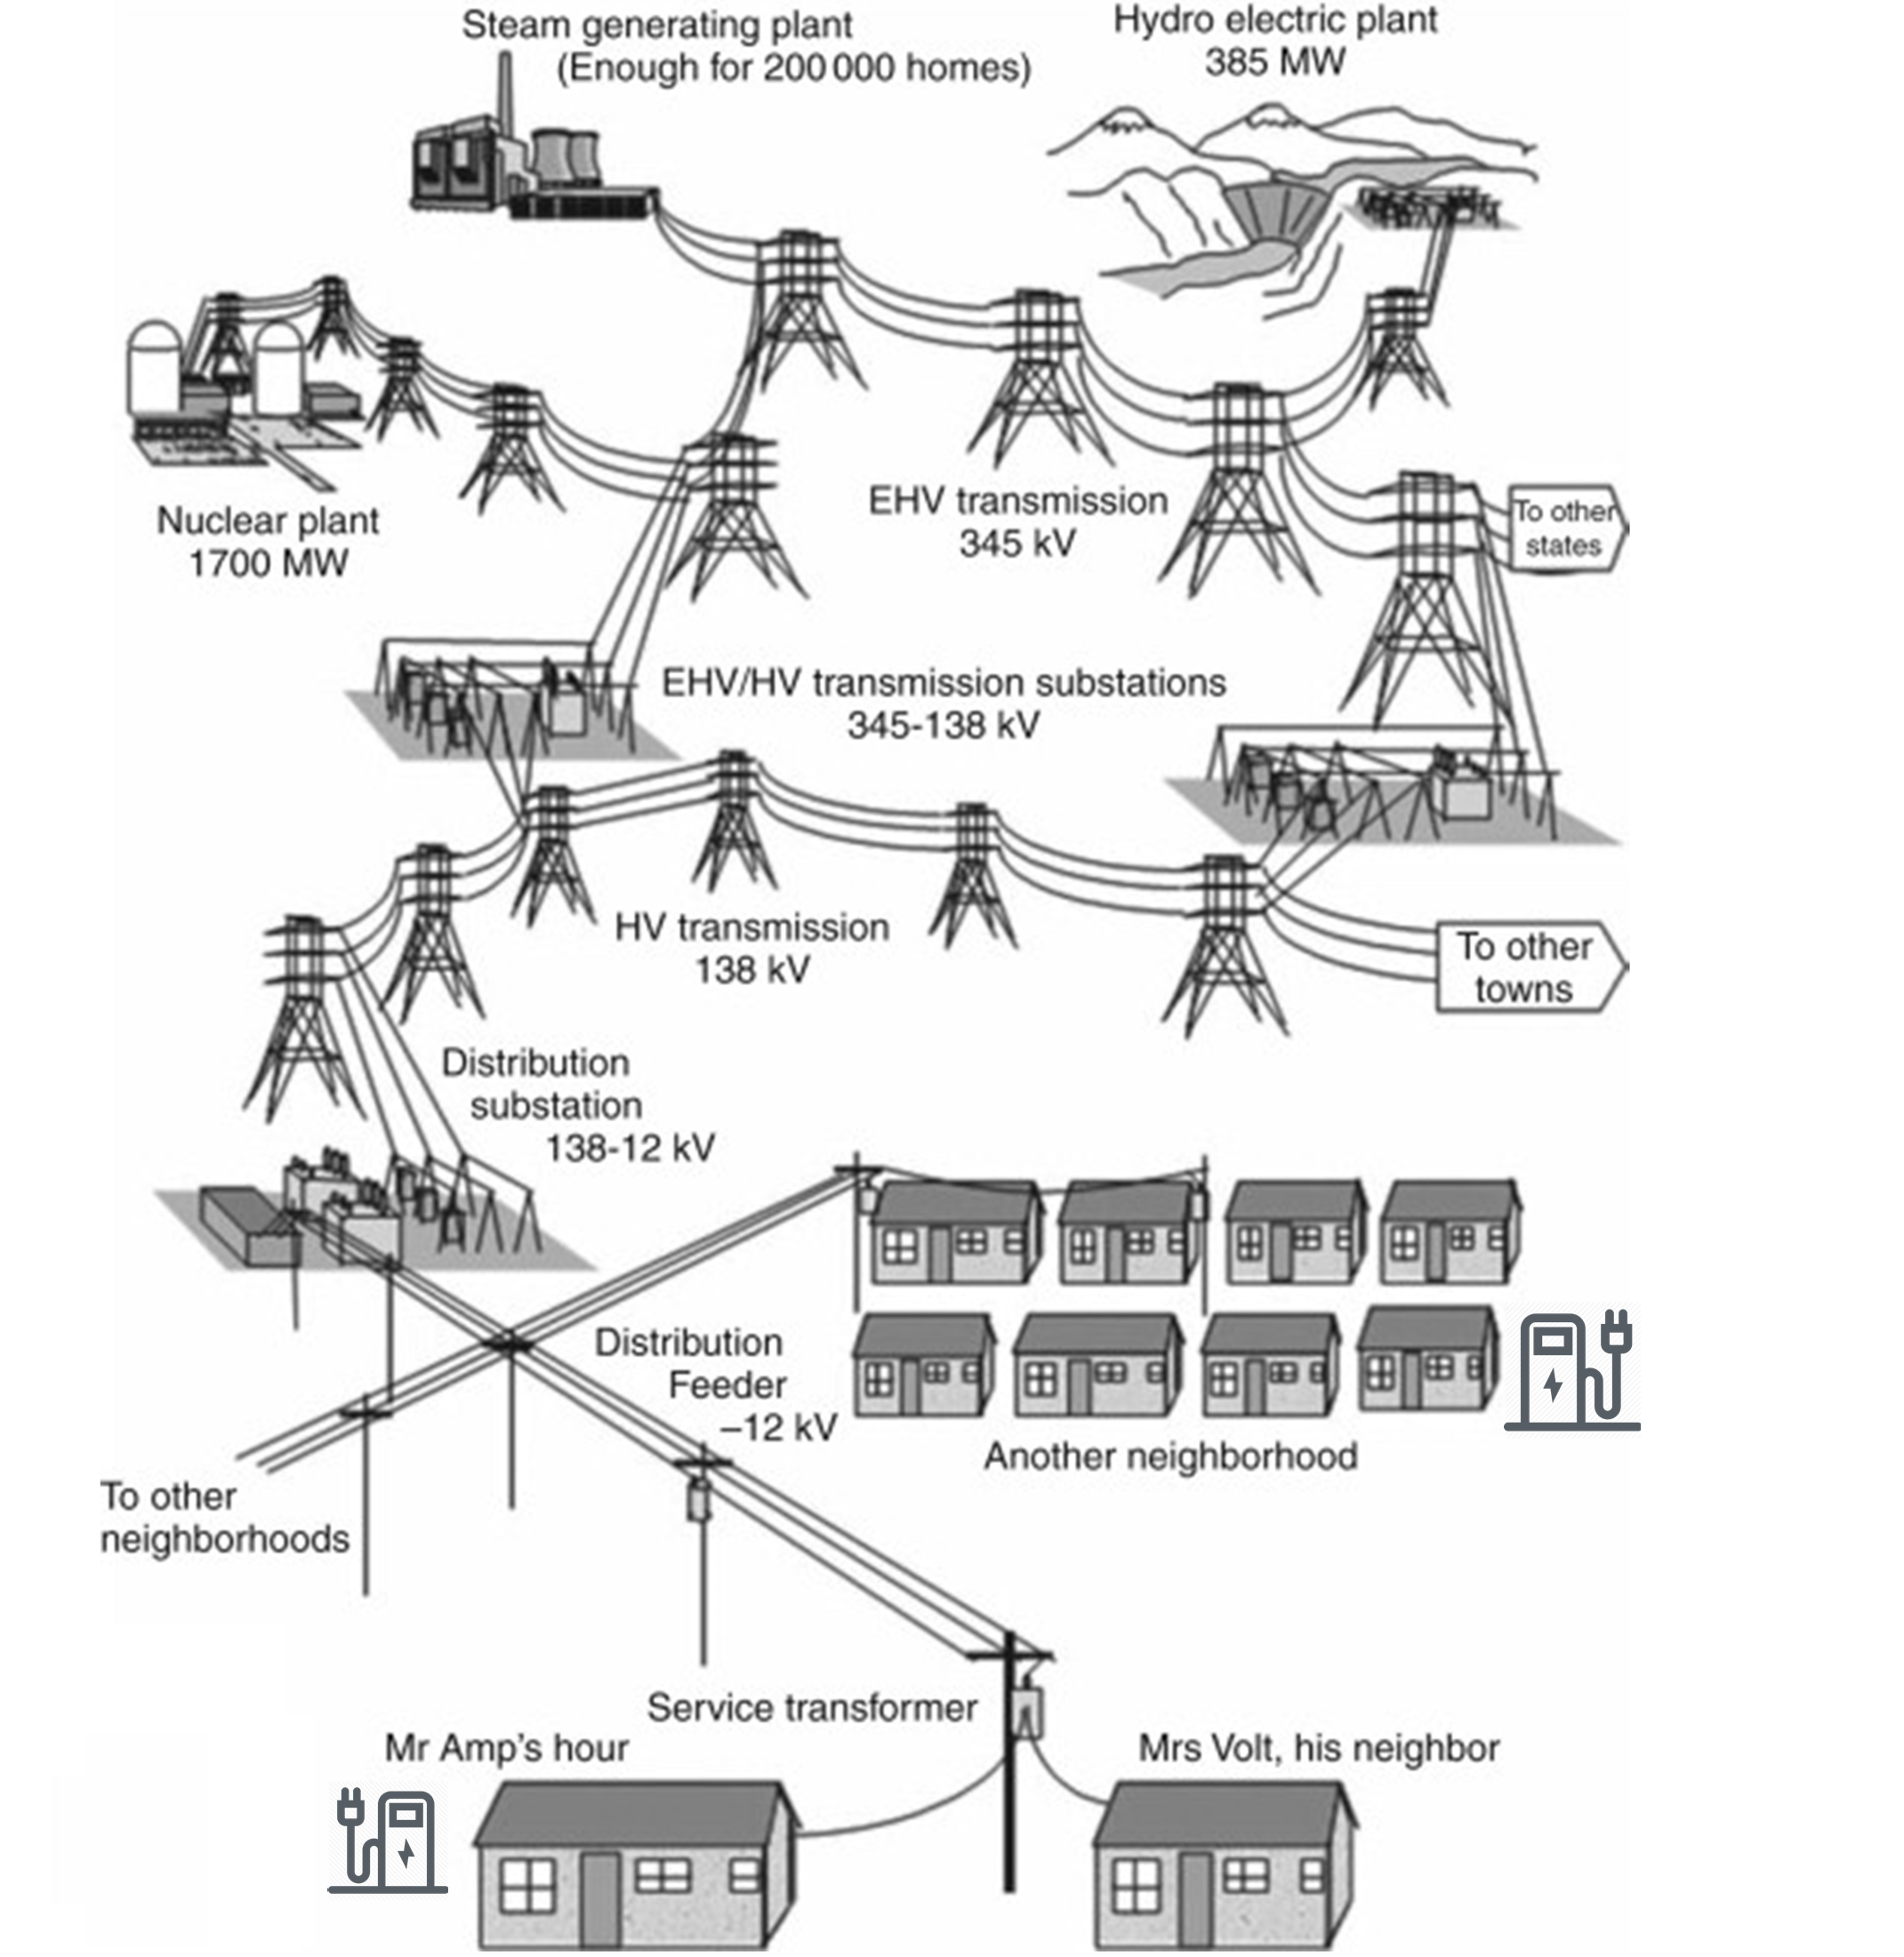
\includegraphics[width=2.8 in , height=2.4 in]{Figures/EVchalendge1.png}
%\caption{\tiny[www.sciencedirect.com/science/article/pii/B9781845697846500019]}
%\end{figure}
%\end{frame}

%%%%%%%%%%%%%%%%%%%%%%%%%%%%%%%%%%%%%%%%%%
%%%%%%%%%%%%%%%%%%%%%%%%%%%%%%%%%%%%%%%%%%
%%%%%%%%%%%%%%%%%%%%%%%%%%%%%%%%%%%%%%%%%%
%%%%%%%%%%%%%%%%%%%%%%%%%%%%%%%%%%%%%%%%%%

\begin{frame}{Sustainability/Green shift/CO\textsubscript{2} reduction}
\begin{alertblock}{\textcolor{red}{For many reasons power electricity grid is facing decentralization}}
\begin{itemize}
\item<1-> Phasing out coal (carbon-heavy sources of production) and nuclear power plants
\item<2-> Increase penetration of solar and wind production
\end{itemize}
\end{alertblock}
\begin{columns}
    \column{0.5\textwidth}
    This chain between large power producers and consumers is weakened.
    \column{0.5\textwidth}
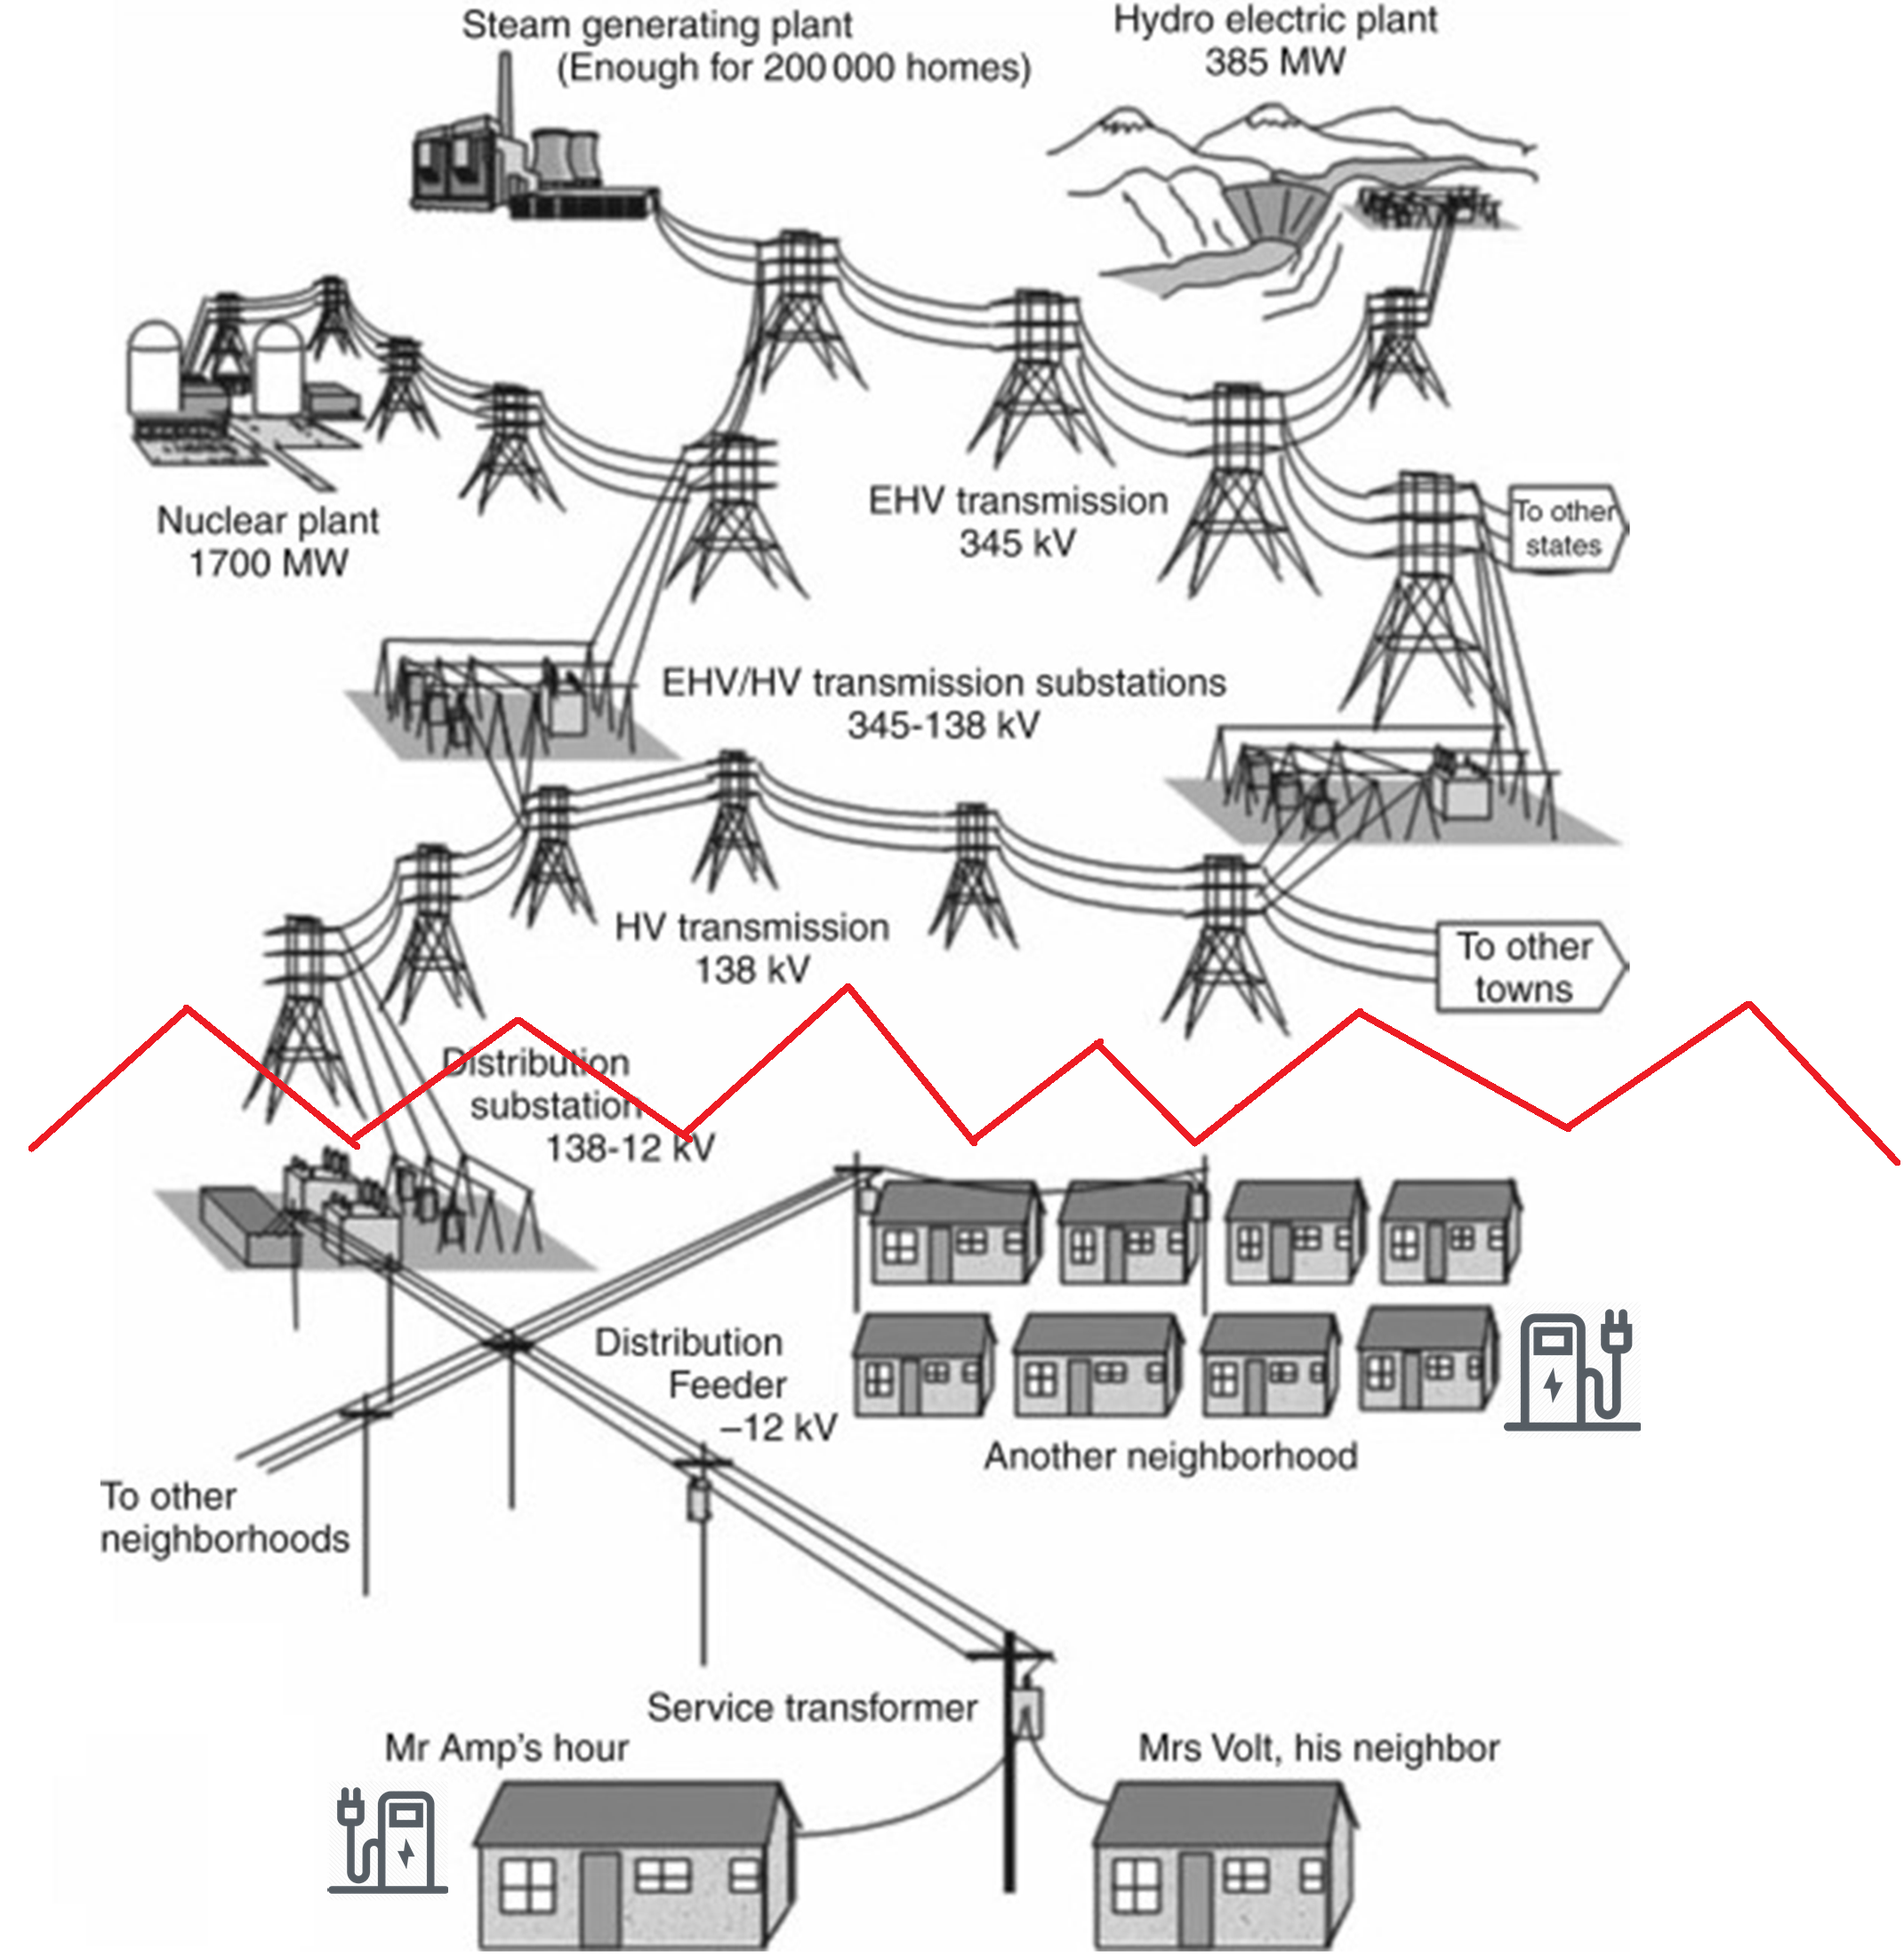
\includegraphics[width=2 in , height=1.6 in]{Figures/EVchalendgebreak.png}
\end{columns}
\end{frame}

%%%%%%%%%%%%%%%%%%%%%%%%%%%%%%%%%%%%%%%%%%
%%%%%%%%%%%%%%%%%%%%%%%%%%%%%%%%%%%%%%%%%%
%%%%%%%%%%%%%%%%%%%%%%%%%%%%%%%%%%%%%%%%%%
%%%%%%%%%%%%%%%%%%%%%%%%%%%%%%%%%%%%%%%%%%
\section{Background}
\begin{frame}{Background: cont.}
\begin{block}{Items}
\begin{itemize}
\item <1-> \small Green shift in electricity systems is needed for the reduction of $\mathrm{CO_2}$ emissions
\begin{itemize}  
\item<2-> \tiny  Integration of Distributed Energy Resources (DER) is a huge challenge
\end{itemize}
\only<2>{ \begin{alertblock}{\tiny Note}
{\tiny DER includes Renewable Energy, Energy Storage, Electric Vehicles and Flexible Demand}
\end{alertblock}}
\item<3->\small Grid companies must be able to analyse the impacts of DER
\only<4>{ \begin{alertblock}{Note}
\textbf{\tiny Optimal Power Flow (OPF)}{\tiny solvers are essential}
\end{alertblock}}
\item<5->\small The inegration of DER in smart grids calls for \textbf{much more sophisticated solvers} for OPF
\end{itemize}
\end{block}
\begin{figure}
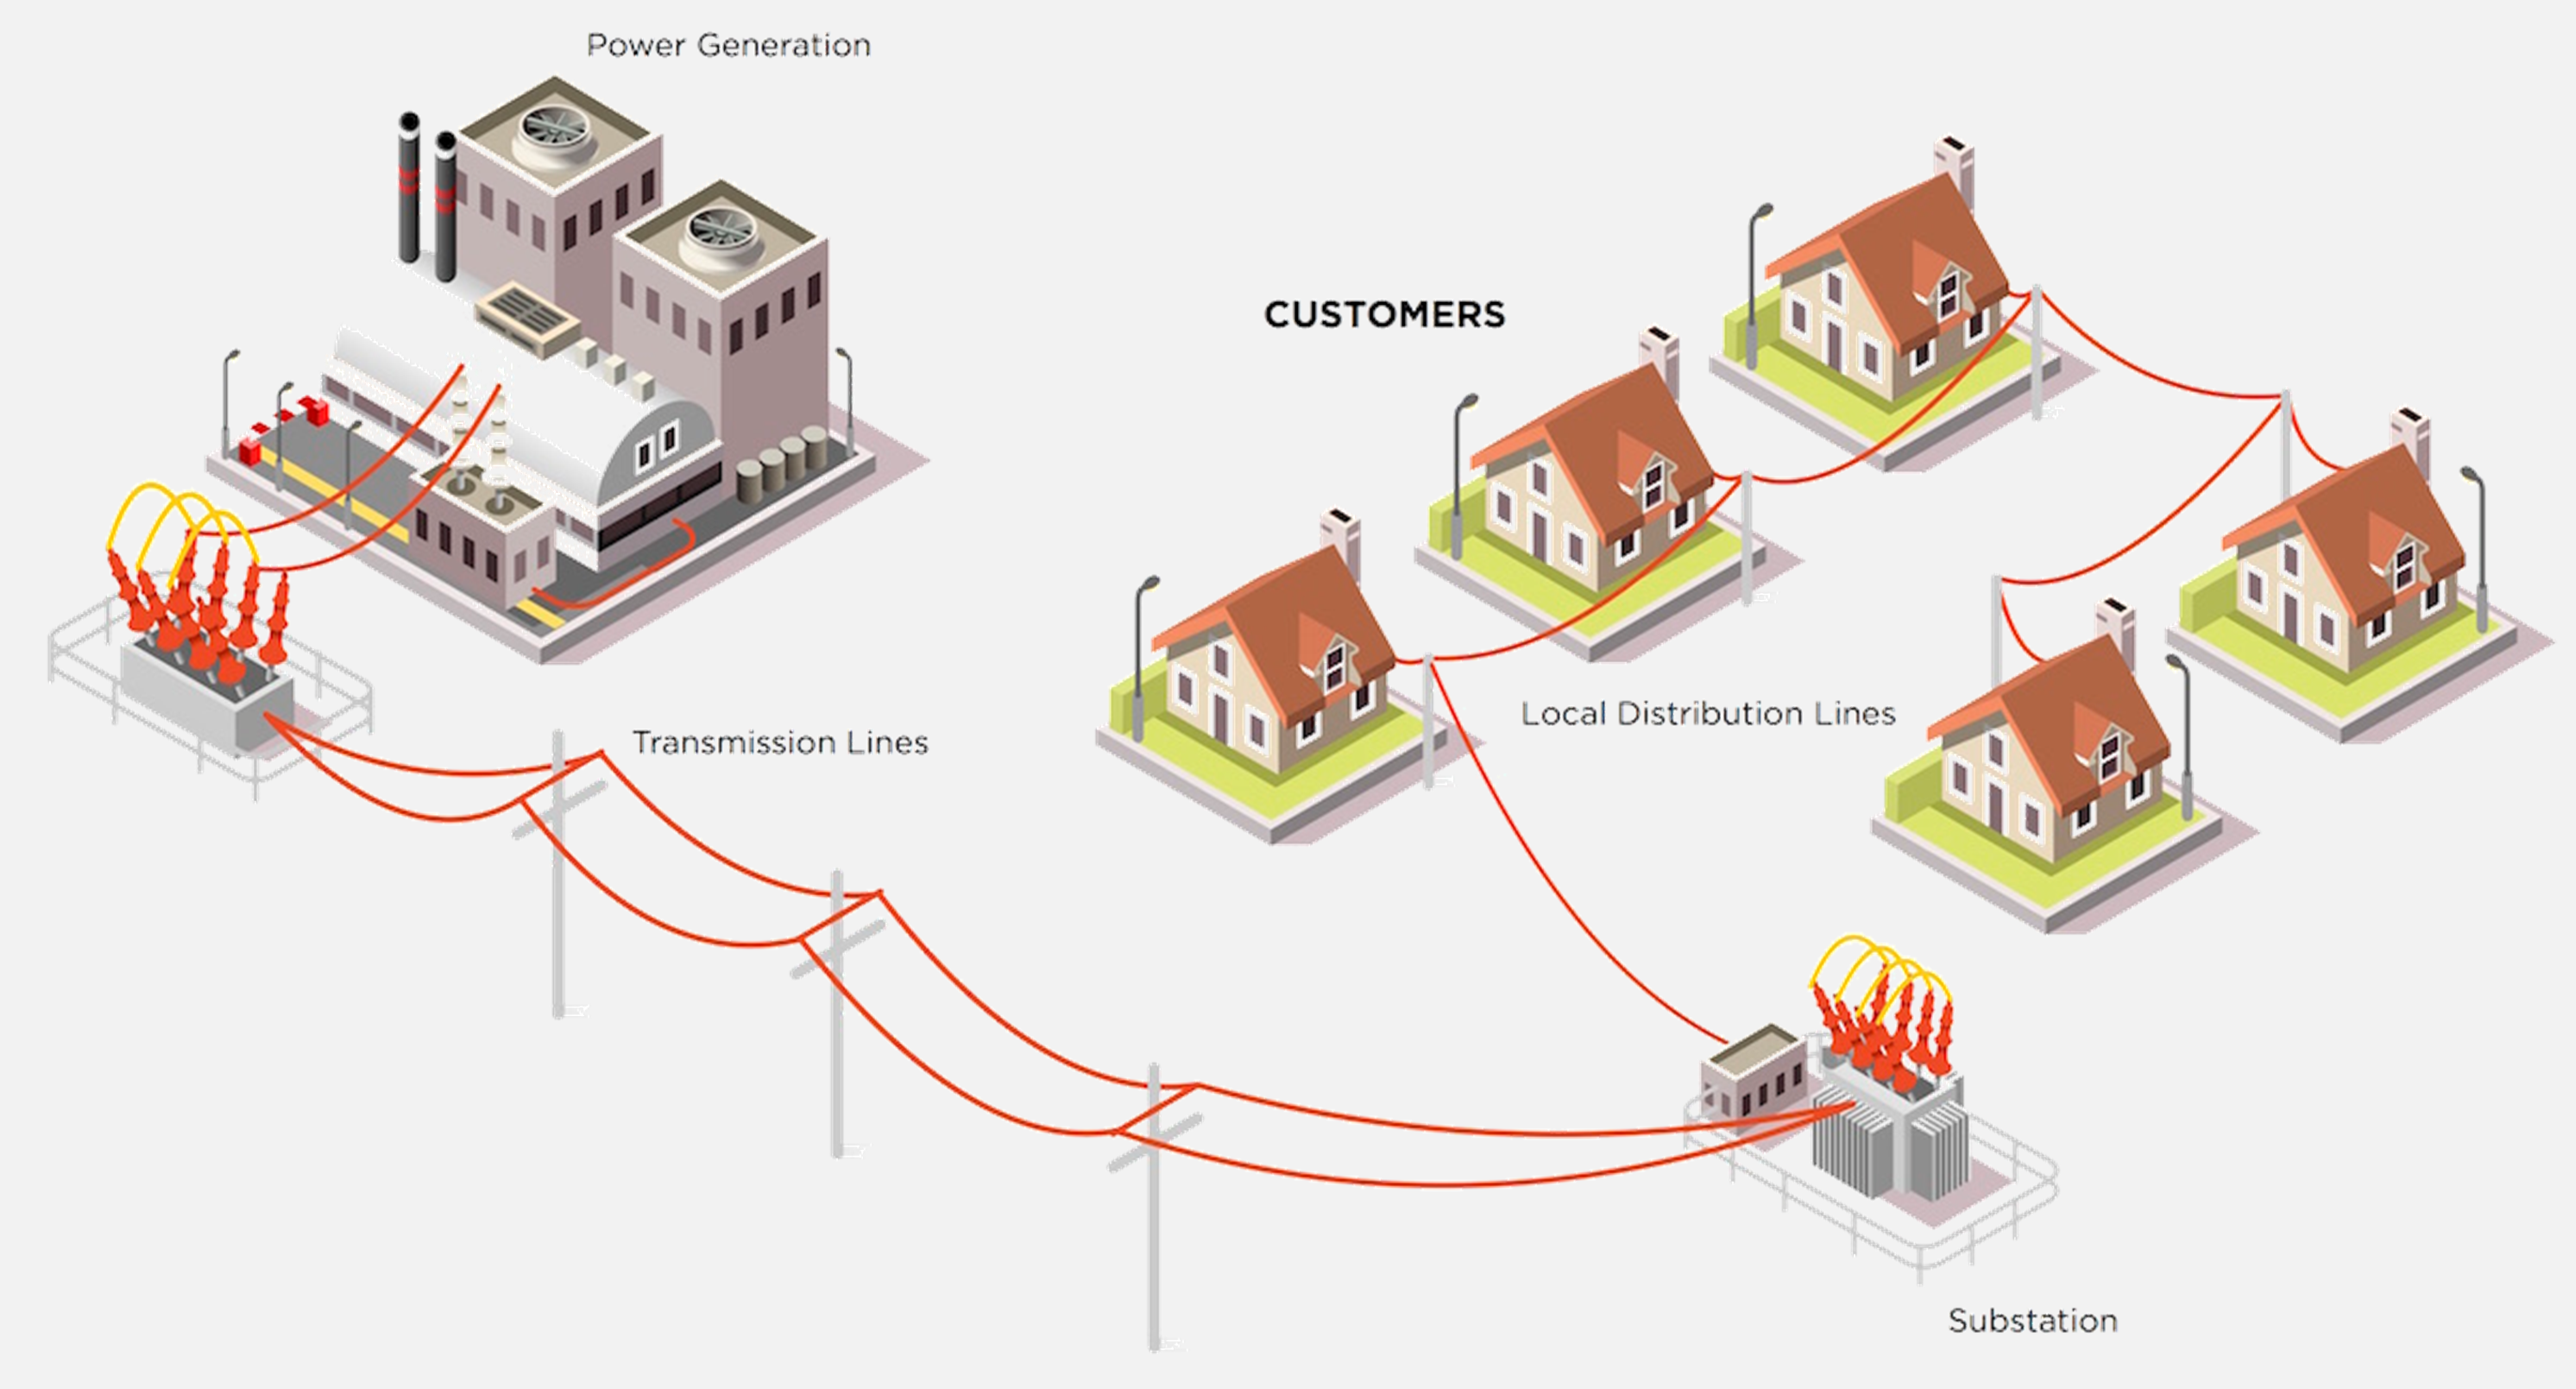
\includegraphics[scale=0.06]{Figures/PowerSys.png}
 \caption{A Typical Power System \textcolor{gray}{\tiny[Rochester Gas \& Electricity]}}
\end{figure}

\end{frame}
        %%%%%%%%%%%%%%%%%%%%%%%%%%%%%%%%%
%%%%%%%%%%%%%%%%%%%%%%%%%%%%%%%%%%%
%%%%%%%%%%%%%%%%%%%%%%%%%%%%%%%%%%%%
%%%%%%%%%%%%%%%%%%%%%%%%%%%%%%%%%%%
%%%%%%%%%%%%%%%%%%%%%%%%%%%%%%%%%
\begin{frame}{Challenges in the planning and operation of the grid}
\begin{itemize}
\item<1-> \textbf{Planning:} Optimizing the right type, size and timing of new grid investments
\begin{itemize}
\item Local generation (e.g. PV) and increased load (e.g. EVs)  can be located in areas where the grid is weak
\item Energy storage and demand flexibility are alternatives to grid reinforcements
\end{itemize}

\item<2-> \textbf{Operation:}Optimize the use of controllable assets such as energy storage and flexible demand to secure, reliable and economic operation of the distribution grids. This means:
\begin{itemize}
\item Making the right use of Demand Response
\item being able to value the use of end-user flexibility for local or system-wide grid services
\item Simulating and optimizing the grids in the presence of \textbf{future local markets for energy and flexibility}
\end{itemize}
\end{itemize}
\end{frame}
%%%%%%%%%%%%%%%%%%%%%%%%%%%%%%%%%
%%%%%%%%%%%%%%%%%%%%%%%%%%%%%%%%%%%
%%%%%%%%%%%%%%%%%%%%%%%%%%%%%%%%%%%%
%%%%%%%%%%%%%%%%%%%%%%%%%%%%%%%%%%%
%%%%%%%%%%%%%%%%%%%%%%%%%%%%%%%%%

\begin{frame}{Limitations of traditional grid operation and planning}
\vskip -1cm
\begin{block}{Notes}
{\scriptsize
\begin{itemize}
\item<1-> Classical single-period OPF does not offer a possibility for optimal operational scheduling of storage and flexible demand
\item<2->  We therefore aim to develop the foundations for a new generation of Multi-Period OPF (MPOPF) solvers
\begin{enumerate}[i.]
{\tiny
\item Solves the OPF problem over several coupled time-steps
\item Computation time is an issue when using both commercial or free optimization solvers
}
\end{enumerate}
\item<3-> MPOPF is an extremely challenging scientific task:
\begin{enumerate}[i.]
{\tiny
\item Nonlinearity
\item Large-scale problem with respect with to time and space
\item Involves stochastic generations and load}
\end{enumerate}
\end{itemize}}
\onslide<4>{\begin{alertblock}{Hardware is reaching its limit with respect to CPU clock speed}
\end{alertblock}}
\end{block}
\begin{backgroundblock}{10mm}{50mm}
 \begin{tikzpicture}
    \node[anchor=east,inner sep=0] (B) at (4,0) {
\includegraphics[scale=0.8]{Figures/CPUSpeed.jpg}};
           \fill [draw=none, fill=white, fill opacity=0.5] (B.north west) -- (B.north east) -- (B.south east) -- (B.south west) -- (B.north west) -- cycle;
    \end{tikzpicture}
   \end{backgroundblock}
\end{frame}
%%%%%%%%%%%%%%%%%%%%%%%%
%%%%%%%%%%%%%%%%%%%%%%%%%%%%%%%%
        %%%%%%%%%%%%%%%%%%%%%%%%%%%%%%%%%
%%%%%%%%%%%%%%%%%%%%%%%%%%%%%%%%%%%
%%%%%%%%%%%%%%%%%%%%%%%%%%%%%%%%%%%%
%%%%%%%%%%%%%%%%%%%%%%%%%%%%%%%%%%%
%%%%%%%%%%%%%%%%%%%%%%%%%%%%%%%%%
\begin{frame}{Solution:}
\begin{block}{High-Performance Solver [1-2]}
\begin{itemize}
\item<1-> Algorithmic design tailored to the conventional OPF algorithms speed-up the solution proposal
\item<1-> Prototype model shows convincing results for real-sized system with distributed renewables, storages and EVs

\begin{enumerate}[i.]
{\tiny
\item A high-performance and memory-efficient sparse algorithm
\item Utilizing the structure of the underlying mathematical formulation}
\end{enumerate}
\end{itemize}
\end{block}

\onslide<2->{\begin{block}{Benefits}
\begin{itemize}
\item<2-> Optimal utilization of \textbf{stored energy} and \textbf{flexibility} where and when it creates the highest value for the system
\item<3-> Can be used for grid planning, grid operation and local markets
\end{itemize}
\end{block}}
\begin{enumerate}
{\tiny
\item S. Zaferanlouei, H. Farahmand, V. V. Vadlamudi, M. Korpås,“BATTPOWER Toolbox: Memory-Efficient and High-Performance Multi-Period AC Optimal Power Flow Solver”, IEEE Transactions on Power Systems, Jan. 16th, 2021.
\item S. Zaferanlouei, et al., “BATTPOWER Application: Large-Scale Integration of EVs in an Active Distribution Grid ---A Norwegian Case Study”, Under review in the journal of EPSR}
 \end{enumerate}
\end{frame}
%%%%%%%%%%%%%%%%%%%%%%%%%%%%%%%%%%%%%%%%%
%%%%%%%%%%%%%%%%%%%%%%%%%%%%%%%%%%%%%%%%%




%%%%%%%%%%%%%%%%%%%%%%%%%%%%%%%
\begin{frame}{Power System--- Today}
\centering
%\animategraphics[loop,width=10cm]{12}{Figures/gif/Today/01-}{0}{115}
\end{frame}
%%%%%%%%%%%%%%%%%%%%%%%%%%%%%%%%%%%%%%%%%%
%%%%%%%%%%%%%%%%%%%%%%%%%%%%%%%%%%%%%%%%%%
%%%%%%%%%%%%%%%%%%%%%%%%%%%%%%%%%%%%%%%%%%
%%%%%%%%%%%%%%%%%%%%%%%%%%%%%%%%%%%%%%%%%%

\begin{frame}{Power System--- Future}
\centering
%\animategraphics[loop,width=10cm]{12}{Figures/gif/Future/01-}{0}{98}
\end{frame}

%%%%%%%%%%%%%%%%%%%%%%%%%%%%%%%%%%%%%%%%%%
%%%%%%%%%%%%%%%%%%%%%%%%%%%%%%%%%%%%%%%%%%
%%%%%%%%%%%%%%%%%%%%%%%%%%%%%%%%%%%%%%%%%%
%%%%%%%%%%%%%%%%%%%%%%%%%%%%%%%%%%%%%%%%%%


\begin{frame}[plain]
\begin{tikzpicture}[overlay, remember picture]
\node[anchor=center] at (current page.center) {
\begin{beamercolorbox}[center]{title}
     Phase II:\\\textbf{Power Flow and Optimal Power Flow}
  \end{beamercolorbox}};
\end{tikzpicture}

\end{frame}

%%%%%%%%%%%%%%%%%%%%%%%%%%%%%%%%% 
%%%%%%%%%%%%%%%%%%%%%%%%%%%%%%%%%%% 
%%%%%%%%%%%%%%%%%%%%%%%%%%%%%%%%%%%% 
%%%%%%%%%%%%%%%%%%%%%%%%%%%%%%%%%%% 
%%%%%%%%%%%%%%%%%%%%%%%%%%%%%%%%% 
\section{Power Flow} 
\begin{frame}{Power Flow Equations} 
\vskip -0.4cm 
 
\begin{block}{Source of Non-linearity} 
\textcolor{red}{Nonlinear relationship} between the voltage phasors and the power injections 
\end{block} 
\vskip -0.5cm 
\begin{table}[htbp!] 
\begin{tabular}{|r l| l|}  
\hline 
\multicolumn{3}{|c|}{ 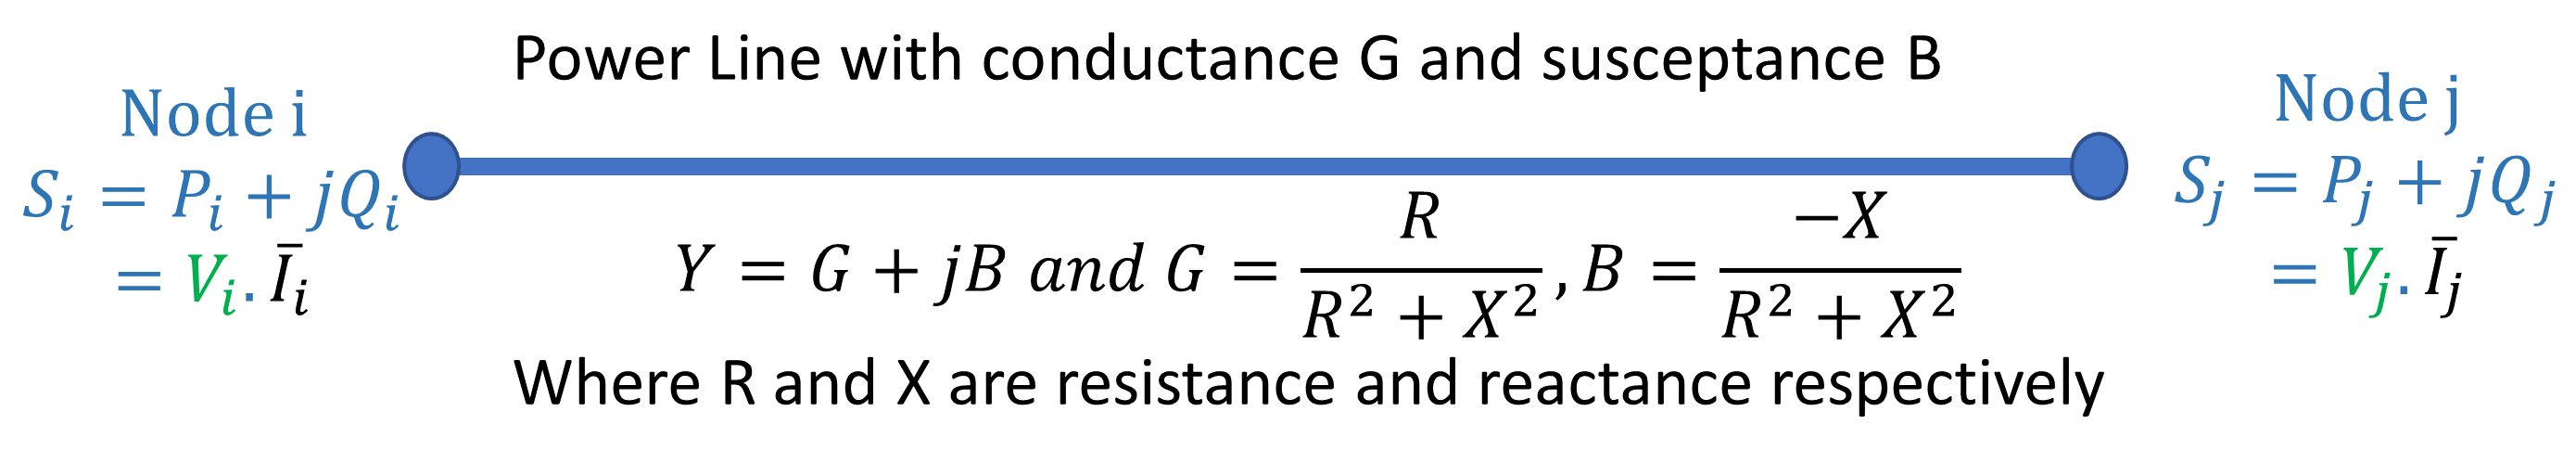
\includegraphics[scale=.15]{Figures/PowerFlow.png}}\\ 
\hline 
 $\textcolor{blue}{P_i}+j\textcolor{blue}{Q_i} $&$= \textcolor{green}{V_i}.\overline{I}_i$& \\ 
 &$=\textcolor{green}{V_i}.(\mathbf{\overline{Y}}_i.\textcolor{green}{\overline{V}})$&{\tiny $\mathbf{{Y}}$ \ admittance matrix}\\ 
 &$=\textcolor{green}{V_i}. (\mathbf{G}_i-j\mathbf{B}_i)\textcolor{green}{\overline{V}}$&{\tiny $\mathbf{{G}}$ and $\mathbf{{B}}$ \  conductance and susceptance matrices}\\ 
 $\textcolor{green}{|V_i|^2}$&$=\textcolor{green}{V_i}.\textcolor{green}{\overline{V}_i}$&{\tiny $\mathbf{{Y}}=\mathbf{G}+j\mathbf{B}$}\\ 
 \multicolumn{2}{|c|}{"Power Flow Equations"}&\\ 
 \multicolumn{2}{|c|}{"Load Flow Equations"}&\\ 
 \hline 
 \end{tabular} 
\end{table} 
\begin{itemize}[label={>}] 
\item \textcolor{red}{Coupled quadratics} in complex voltage phasors 
\end{itemize} 
\end{frame} 
 
%%%%%%%%%%%%%%%%%%%%%%%%%%%%%%%%% 
%%%%%%%%%%%%%%%%%%%%%%%%%%%%%%%%%%% 
%%%%%%%%%%%%%%%%%%%%%%%%%%%%%%%%%%%% 
%%%%%%%%%%%%%%%%%%%%%%%%%%%%%%%%%%%
%%%%%%%%%%%%%%%%%%%%%%%%%%%%%%%%%
\begin{frame}{Power Flow Equations in Different Coordinates}

\onslide<1-2>{\scriptsize {The \textcolor{red}{bus injection} model
\begin{center}
\begin{tabular}{|c c|}
\hline
\multicolumn{2}{|c|}{ 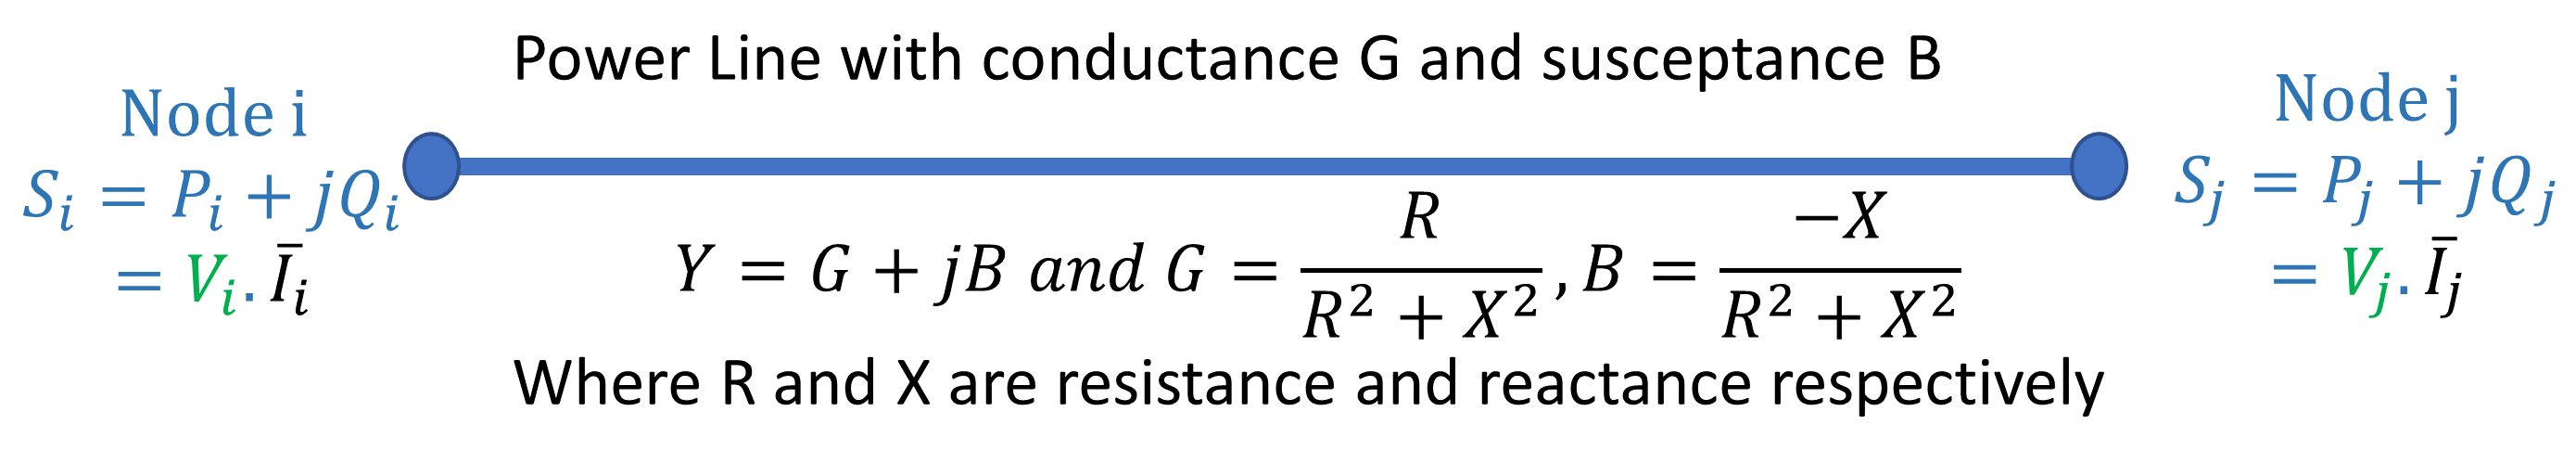
\includegraphics[scale=.15]{Figures/PowerFlow.png}}\\
\hline
 \multicolumn{1}{|c|}{Polar Voltage Coordinates}&$\textcolor {green}{V_i}=\textcolor {green}{\abs{V_i}}\angle \textcolor {green}{\theta_i}$\quad $\textcolor {green}{\theta_1}=0$\\
\cline{1-1}
\multicolumn{2}{|c|}{$ 
 \textcolor {blue}{P_{i}} =\textcolor {green}{\abs{V_{i}}}\sum_{j=1}^{N} \textcolor {green}{\abs{V_{j}}} (\boldsymbol{G}_{ij} cos(\textcolor {green}{\theta{i}}-\textcolor {green}{\theta{j}})+\boldsymbol{B}_{ij}sin(\textcolor {green}{\theta{i}}-\textcolor {green}{\theta{j}}))$}\\

\multicolumn{2}{|c|}{$ \textcolor {blue}{Q_{i}} =\textcolor {green}{\abs{V_{i}}}\sum_{j=1}^{N}
 \textcolor {green}{\abs{V_{j}}} (\boldsymbol{G}_{ij} sin(\textcolor {green}{\theta{i}}-\textcolor {green}{\theta{j}})-\boldsymbol{B}_{ij}cos(\textcolor {green}{\theta{i}}-\textcolor {green}{\theta{j}}))$}\\
 \hline\hline
  \multicolumn{1}{|c|}{Rectangular Voltage Coordinates}&$\textcolor {green}{V_i}=\textcolor {green}{V_{di}}+j \textcolor {green}{V_{qi}}$\quad $\textcolor {green}{V_{q1}}=0$\\
\cline{1-1}
\multicolumn{2}{|c|}{$ 
 \textcolor {blue}{P_{i}} =\textcolor {green}{V_{di}}(\boldsymbol{G}_{ij} \textcolor {green}{V_{dj}} -\boldsymbol{B}_{ij} \textcolor {green}{V_{qj}})
 +
 \textcolor {green}{V_{qi}}(\boldsymbol{B}_{ij} \textcolor {green}{V_{dj}} +\boldsymbol{G}_{ij} \textcolor {green}{V_{qj}})$}\\

\multicolumn{2}{|c|}{$ 
 \textcolor {blue}{Q_{i}} =-\textcolor {green}{V_{di}}(\boldsymbol{B}_{ij} \textcolor {green}{V_{dj}} +\boldsymbol{G}_{ij} \textcolor {green}{V_{qj}})
 +
 \textcolor {green}{V_{qi}}(\boldsymbol{G}_{ij} \textcolor {green}{V_{dj}} -\boldsymbol{B}_{ij} \textcolor {green}{V_{qj}})$}\\

$ \textcolor {green}{V_{di}}= Re (\textcolor {green}{V_i})$ \  $ \textcolor {green}{V_{qi}}= Im (\textcolor {green}{V_i})$& $N=$ number of Nodes\\
  \hline
\end{tabular}
\end{center}}}
\onslide<2-> {\scriptsize \begin{block}{Power Flow}
PF equations are a set of nonlinear algebraic equations which can be solved with Newton-Raphson, Gauss–Seidel, Fast-decoupled-load-flow method and etc.
\end{block}}

\end{frame}

%%%%%%%%%%%%%%%%%%%%%%%%%%%%%%%%%%%%
%%%%%%%%%%%%%%%%%%%%%%%%%%%%%%%%%%%
%%%%%%%%%%%%%%%%%%%%%%%%%%%%%%%%%
\subsection{Single Period ACOPF}
\begin{frame}{Single period ACOPF - problem formulation}
\begin{block}{Single Period AC Optimal Power Flow (ACOPF)}
We are controlling some variables in OPF to minimise system costs with respect to constraints.
\end{block}
\begin{center}
\begin{tabular}{|l l|}
\hline
Objective Function&$\min_{\mathbf{x}} f(\mathbf{x})$\\
\rowcolor{Gray}
\begin{tabular}[l]{@{}l@{}}Equality Constraints\\ (Balance)\\ Power Flow \end{tabular}  &$\textrm{s.t. }  \mathbf{g}(\mathbf{x})= \begin{colorbmatrix}
   \mathbf{\widetilde{g}}(\mathbf{x})\\
   \mathbf{\overline{g}}(\mathbf{x})
\end{colorbmatrix}=0 \qquad \in   \mathbb{R}^{n_{gx} \times 1}$\\

\begin{tabular}[l]{@{}l@{}}Inequality constraints\\ (line and transformer)\\ Operational Constraints \end{tabular}  & $\mathbf{h}(\mathbf{x})=\begin{colorbmatrix}
   \mathbf{\widetilde{h}}(\mathbf{x})\\
   \mathbf{\overline{h}}(\mathbf{x})
\end{colorbmatrix}\leq 0 \qquad \in   \mathbb{R}^{n_{hx} \times 1} $\\
\rowcolor{Gray}
Vector of Variables&$ \mathbf{x}= \big[\boldsymbol{\Theta}\  \boldsymbol{\mathcal{V}} \  \boldsymbol{\mathcal{P}}^{\mathrm{g}} \ \boldsymbol{\mathcal{Q}}^{\mathrm{g}} \big]^\top
 \in \mathbb{R}^{n_{x}\times 1}$\\
\hline
\end{tabular}
\end{center}
\end{frame}
%%%%%%%%%%%%%%%%%%%%%%%%%%%%%%%%%
%%%%%%%%%%%%%%%%%%%%%%%%%%%%%%%%%%%
%%%%%%%%%%%%%%%%%%%%%%%%%%%%%%%%%%%%
\subsection{Limitations of PF and single period OPF}
\begin{frame}
\onslide<1->
{\footnotesize
\begin{block}{Limitation of Power Flow}
\begin{tabular}{|l|}
\hline
\rowcolor{Gray}
\tabitem PF is only a set of static equations which provides status of a system\\
 \rowcolor{Gray}\qquad for time: $t=t_s$\\
\rowcolor{Gray} \tabitem It does not include  generation constraints and operational constraints\\
\hline
\end{tabular}
\end{block}
}
\onslide<2->
{\footnotesize
\begin{block}{
Limitation of Single Period AC Optimal Power Flow}

\begin{tabular}{|l|}
\hline
\rowcolor{Gray} \quad \tabitem OPF is an optimisation problem which optimises status of a system\\
\rowcolor{Gray}\ \ \qquad for a SINGLE time: $t=t_s$.\\
\rowcolor{Gray} \quad \tabitem Although it includes the operational constraints for single time,\\
\rowcolor{Gray}  \qquad it will not include operation of DERs and generators over a time horizon.\\
\rowcolor{Gray} \quad \tabitem It is not capable of integrating storage devices and EVs. \\
\hline
\end{tabular}
}
\end{block}
\onslide<3->
\begin{alertblock}
{ Our suggested approach: multi-period ACOPF}
{ Solves the OPF problem over several time-steps at once useful formulation for systems with Energy Storage and Shiftable Loads (e.g. Evs)}
\end{alertblock}
\end{frame}
%%%%%%%%%%%%%%%%%%%%%%%%%%%%%%%%%
%%%%%%%%%%%%%%%%%%%%%%%%%%%%%%%%%%%
%%%%%%%%%%%%%%%%%%%%%%%%%%%%%%%%%%%%
%%%%%%%%%%%%%%%%%%%%%%%%%%%%%%%%%%%
%%%%%%%%%%%%%%%%%%%%%%%%%%%%%%%%%
\subsection{MultiPeriod ACOPF}
\begin{frame}
\onslide<1->{
\begin{block}{Advantages of MultiPeriod ACOPF}
\textcolor{red}{>} Integrating dependent time power system's components such as stationary ESS, EV, generators ramp rate, and so on.\\}
\onslide<2-> {\textcolor{red}{>} between 2\% to 5\% less costly solutions.
\only<2>{\begin{backgroundblock}{50mm}{45mm}
        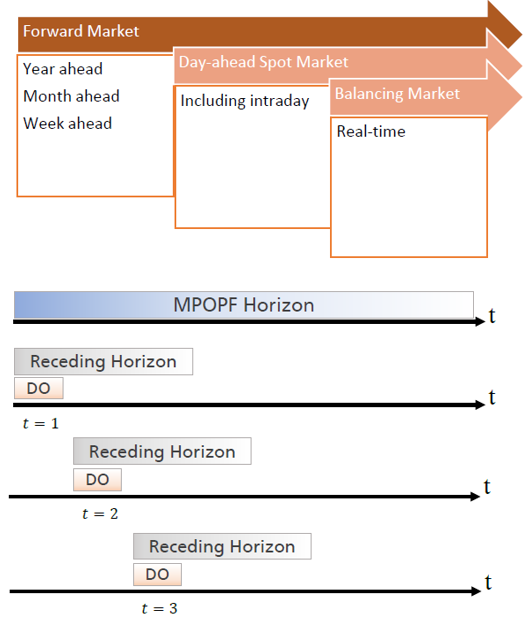
\includegraphics[scale=0.33]{Figures/ReceedingHorizon.png}
        \end{backgroundblock}}
\end{block}}
\visible<3-> {\begin{block}{Disadvantage of MultiPeriod ACOPF}
The problem grows very large as the number of time-steps is increased, which may lead to an intractable solution.
\end{block}}
\end{frame}
%%%%%%%%%%%%%%%%%%%%%%%%%%%%%%%%%%%
%%%%%%%%%%%%%%%%%%%%%%%%%%%%%%%%%%%%
%%%%%%%%%%%%%%%%%%%%%%%%%%%%%%%%%%%
%%%%%%%%%%%%%%%%%%%%%%%%%%%%%%%%%
\begin{frame}{MultiPeriod ACOPF-problem formulation}
\begin{center}
\begin{tabular}{|l l|}
\hline
{\tiny Objective Function}&$\min_{\mathbf{X}} F(\mathbf{X})$\\
\rowcolor{Gray}
{\tiny \begin{tabular}[l]{@{}l@{}}Equality Constraints\\ (Balance)\\ Power Flow \end{tabular} } &$\textrm{s.t. } G(\mathbf{X})= \begin{colorbmatrix}
   \widetilde{G}(\mathbf{X}) \
   \overline{G}(\mathbf{X}) \
   \overline{G}^s(\mathbf{X})
\end{colorbmatrix}^\top=0  \in   \mathbb{R}^{N_{g} \times 1}$\\

{\tiny \begin{tabular}[l]{@{}l@{}}Inequality constraints\\ (line and transformer)\\ Operational Constraints \end{tabular} } & $H(\mathbf{X})=\begin{colorbmatrix}
   \widetilde{H}(\mathbf{X}) \quad
   \overline{H}(\mathbf{X})
\end{colorbmatrix}^\top\leq 0  \in   \mathbb{R}^{N_{h} \times 1} $\\
\rowcolor{Gray}
{\tiny Vectors of Constraints}&{\tiny \begin{tabular}[l]{@{}l@{}}$
   \widetilde{\mathbf{G}}(\mathbf{X})=
\begin{colorbmatrix}
    \widetilde{\mathbf{g}}(\mathbf{x}_{1}) \
    \widetilde{\mathbf{g}}(\mathbf{x}_{2}) \
    \dots \
    \widetilde{\mathbf{g}}(\mathbf{x}_{T}) 
\end{colorbmatrix}^\top$\\ $ 
   \overline{\mathbf{G}}(\mathbf{X})=
\begin{colorbmatrix}
    \overline{\mathbf{g}}(\mathbf{x}_{1}) \
    \overline{\mathbf{g}}(\mathbf{x}_{2}) \
    \dots \
    \overline{\mathbf{g}}(\mathbf{x}_{T}) \
\end{colorbmatrix}^\top $\\ $
  \overline{\mathbf{G}}^s(\mathbf{X})=
\begin{colorbmatrix}
    \overline{\mathbf{g}}^s(\boldsymbol{\tau}_1) \
    \overline{\mathbf{g}}^s(\boldsymbol{\tau}_2) \
    \dots \
    \overline{\mathbf{g}}^s(\boldsymbol{\tau}_T) 
\end{colorbmatrix}^\top  $\\ $
   \widetilde{\mathbf{H}}(\mathbf{X})=
\begin{colorbmatrix}
    \widetilde{\mathbf{h}}(\mathbf{x}_{1}) \
    \widetilde{\mathbf{h}}(\mathbf{x}_{2}) \
    \dots \
    \widetilde{\mathbf{h}}(\mathbf{x}_{T}) 
\end{colorbmatrix}^\top$\\ $
  \overline{\mathbf{H}}(\mathbf{X})= 
\begin{colorbmatrix}
    \overline{\mathbf{h}}(\mathbf{x}_{1}) \
    \overline{\mathbf{h}}(\mathbf{x}_{2}) \
    \dots \
    \overline{\mathbf{h}}(\mathbf{x}_{T}) 
\end{colorbmatrix}^\top $\end{tabular}  
}\\  
\hline
\end{tabular}
\end{center}



\end{frame}
%%%%%%%%%%%%%%%%%%%%%%%%%%%%%%%%%
%%%%%%%%%%%%%%%%%%%%%%%%%%%%%%%%%%%
%%%%%%%%%%%%%%%%%%%%%%%%%%%%%%%%%%%%
%%%%%%%%%%%%%%%%%%%%%%%%%%%%%%%%%%%
%%%%%%%%%%%%%%%%%%%%%%%%%%%%%%%%%

%%%%%%%%%%%%%%%%%%%
%%%%%%%%%%%%%%%
\begin{frame}[plain]
\begin{tikzpicture}[overlay, remember picture]
\node[anchor=center] at (current page.center) {
\begin{beamercolorbox}[center]{title}
     Phase III:\\\textbf{Solution Methods}
  \end{beamercolorbox}};
\end{tikzpicture}

\end{frame}
%%%%%%%%%%%%%%%%%%%%%%%%%%%%%%%%%
%%%%%%%%%%%%%%%%%%%%%%%%%%%%%%%%%%%
%%%%%%%%%%%%%%%%%%%%%%%%%%%%%%%%%%%%
%%%%%%%%%%%%%%%%%%%%%%%%%%%%%%%%%%%
%%%%%%%%%%%%%%%%%%%%%%%%%%%%%%%%%
\section{Solution Method}
\begin{frame}{Nonlinear Programming (NLP)}
\begin{block}{How do we solve Optimal Power Flow?}
\begin{enumerate}[I.]
\item<1-> Interior Point Method
\item<2-> Gradient Decent Method
\item<3-> Heuristic Methods
\end{enumerate}
\end{block}
\onslide<4>{\begin{alertblock}
{Interior Point Method}
The focus of this study is the interior point method solution
\end{alertblock}}
\end{frame}
%%%%%%%%%%%%%%%%%%%%%%%%%%%%%%%%%
%%%%%%%%%%%%%%%%%%%%%%%%%%%%%%%%%%%
%%%%%%%%%%%%%%%%%%%%%%%%%%%%%%%%%%%%
%%%%%%%%%%%%%%%%%%%%%%%%%%%%%%%%%%%
%%%%%%%%%%%%%%%%%%%%%%%%%%%%%%%%%

%%%%%%%%%%%%%%%%%%%%%%%%%%%%%%%%%
%%%%%%%%%%%%%%%%%%%%%%%%%%%%%%%%%%%
%%%%%%%%%%%%%%%%%%%%%%%%%%%%%%%%%%%%
%%%%%%%%%%%%%%%%%%%%%%%%%%%%%%%%%%%
%%%%%%%%%%%%%%%%%%%%%%%%%%%%%%%%%

\begin{frame}

\begin{center}
\begin{tabular}{|l|}
\hline
\rowcolor{yellow}
Step(1): Applying Slack variables and the barrier term: \\
\rowcolor{Gray}

$\min_{\mathbf{X}} \bigg[F(\mathbf{X})-\gamma\sum_{i=1}^{N_h}{ln(z_{i})}\bigg]$\\ \rowcolor{Gray}

 $\textrm{s.t. }  \mathbf{G}(\mathbf{X})=0$\\ \rowcolor{Gray}

$\mathbf{H}(\mathbf{X})+\mathbf{Z}=0$\\ \rowcolor{Gray}

 $\mathbf{Z}\geq 0$\\
\hline
slack variables "Z" convert inequality constraints\\
 to equality constraints.\\
\hline
\end{tabular}
\end{center}

\end{frame}

%%%%%%%%%%%%%%%%%%%%%%%%%%%%%%%%%
%%%%%%%%%%%%%%%%%%%%%%%%%%%%%%%%%%%
%%%%%%%%%%%%%%%%%%%%%%%%%%%%%%%%%%%%
%%%%%%%%%%%%%%%%%%%%%%%%%%%%%%%%%%%
\begin{frame}
\begin{center}
\begin{tabular}{|l l|}
\hline
\rowcolor{cyan} \multicolumn{2}{|l|}{Step (2): Calculate and form the Lagrangian of Barrier subproblem} \\
\rowcolor{Gray} \multicolumn{2}{|l|}{ $\boldsymbol{\mathcal{L}}^{\gamma}(\mathbf{X},\mathbf{Z},\boldsymbol{\lambda},\boldsymbol{\mu})=f(\mathbf{X})+\boldsymbol{\lambda}^\top \mathbf{G}(\mathbf{X})
+\boldsymbol{\mu}^\top(\mathbf{H}(\mathbf{X})+\mathbf{Z})-\gamma \sum_{i=1}^{N_g}{ln(z_{i})}$}\\
\hline
\multicolumn{2}{l}{}\\
\multicolumn{2}{l}{}\\
\hline
\rowcolor{magenta}
\multicolumn{2}{|l|}{Step (3): Calculate the KKT\footnote{Karush–Kuhn–Tucker conditions} of the Lagrangian}\\
\rowcolor{Gray}
\begin{tabular}[l]{@{}l@{}}Step (3)\\$KKT_X$  \end{tabular} &$\boldsymbol{\mathcal{L}}_{\mathbf{X}}^{\gamma}(\mathbf{X},\mathbf{Z},\boldsymbol{\lambda},\boldsymbol{\mu})=f_{\mathbf{X}}+\boldsymbol{\lambda}^\top \mathbf{G}_{\mathbf{X}}+\boldsymbol{\mu}^\top \mathbf{H}_{\mathbf{X}}=0$\\
\rowcolor{Gray}
\begin{tabular}[l]{@{}l@{}}Step (3)\\$KKT_Z$  \end{tabular}&$\boldsymbol{\mathcal{L}}_{\mathbf{Z}}^{\gamma}(\mathbf{X},\mathbf{Z},\boldsymbol{\lambda},\boldsymbol{\mu})=\boldsymbol{\mu}^\top - \gamma \mathbf{e}^\top\mathbf{diag}(\mathbf{Z})^{-1}=0$\\
\rowcolor{Gray}
\begin{tabular}[l]{@{}l@{}}Step (3)\\$KKT_\lambda$   \end{tabular}  &$\boldsymbol{\mathcal{L}}_{\boldsymbol{\lambda}}^{\gamma}(\mathbf{X},\mathbf{Z},\boldsymbol{\lambda},\boldsymbol{\mu})=\mathbf{G}^\top (\mathbf{X})=0$
\\
  \rowcolor{Gray}
\begin{tabular}[l]{@{}l@{}}Step (3)\\$KKT_\mu$   \end{tabular}    & $
\boldsymbol{\mathcal{L}}_{\boldsymbol{\mu}}^{\gamma}(\mathbf{X},\mathbf{Z},\boldsymbol{\lambda},\boldsymbol{\mu})=\mathbf{H}^\top(\mathbf{X})+\mathbf{Z}^\top=0$\\
\hline
\end{tabular}
\end{center}


\end{frame}
%%%%%%%%%%%%%%%%%%%%%%%%%%%%%%%%%
%%%%%%%%%%%%%%%%%%%%%%%%%%%%%%%%%%%
%%%%%%%%%%%%%%%%%%%%%%%%%%%%%%%%%%%
%%%%%%%%%%%%%%%%%%%%%%%%%%%%%%%%%


\begin{frame}

\begin{center}
\begin{tabular}{|l l|}
\hline
\begin{tabular}[l]{@{}l@{}}Nonlinear \\Algebric \\Equations  \end{tabular} &$\boldsymbol{\Omega}(\mathbf{X},\mathbf{Z},\boldsymbol{\lambda},\boldsymbol{\mu})
=\begin{bmatrix}
    f_{\mathbf{X}}+\boldsymbol{\lambda}^\top \mathbf{G}_{\mathbf{X}}+\boldsymbol{\mu}^\top \mathbf{H}_{\mathbf{X}} \\
   \mathbf{diag}(\mathbf{Z})\boldsymbol{\mu}^\top - \gamma \mathbf{e}^\top\\
    \mathbf{G}^\top (\mathbf{X})\\
    \mathbf{H}^\top(\mathbf{X})+\mathbf{Z}^\top
\end{bmatrix}=0$\\

$S.t.$&$\quad \mathbf{Z} > 0$\\

&$\quad \boldsymbol{\mu} > 0$\\
\hline
\multicolumn{2}{l}{}\\
\hline
\rowcolor{green}
\multicolumn{2}{|l|}{Step (4): Apply Newton Raphson Method}\\
\rowcolor{Gray}
\multicolumn{2}{|l|}{ \quad $[\boldsymbol{\Omega}_\mathbf{X} \ \boldsymbol{\Omega}_\mathbf{Z} \ \boldsymbol{\Omega}_{\boldsymbol{\lambda}} \ \boldsymbol{\Omega}_{\boldsymbol{\mu}}]^k{[\Delta \mathbf{X} \ \Delta \mathbf{Z} \ \Delta \boldsymbol{\lambda} \ \Delta \boldsymbol{\mu}]^\top}^k=-\boldsymbol{\Omega}(\mathbf{X},\mathbf{Z},\boldsymbol{\lambda},\boldsymbol{\mu})^k$}\\
\hline
\end{tabular}
\end{center}

\end{frame}

%%%%%%%%%%%%%%%%%%%%%%%%%%%%%%%%%
%%%%%%%%%%%%%%%%%%%%%%%%%%%%%%%%%%%
\begin{frame}
\begin{center}
\begin{tabular}{|l l|}
\hline
\begin{tabular}[l]{@{}l@{}}Step (5): \\{Inverse Jacobian} \\ of Newton Raphson  \end{tabular} \cellcolor{red} & \cellcolor{Gray}${\textcolor{red}{\begin{colorbmatrix}
    \mathbf{M}&  \mathbf{G}_{\mathbf{X}}^\top\\
    \mathbf{G}_{\mathbf{X}} & 0\\
\end{colorbmatrix}}}^k
{\begin{colorbmatrix}
    \Delta \mathbf{X}\\
   \Delta\boldsymbol{\lambda}
\end{colorbmatrix}}^k=
{\begin{colorbmatrix}
    -\mathbf{N}\\
   -\mathbf{G}(\mathbf{X})
\end{colorbmatrix}}^k $\\
\hline
\end{tabular}
\end{center}
$\mathbf{M} \in \mathbb{R}^{N_x \times N_x}$ and $\mathbf{N} \in \mathbb{R}^{N_x \times 1}$ are defined as:


\begin{center}
\begin{tabular}{|l l|}
\hline
&$ \mathbf{M}=\boldsymbol{\mathcal{L}}_{\mathbf{X}\mathbf{X}}^{\gamma}+\mathbf{H}_{\mathbf{X}}^\top\mathbf{diag}(\mathbf{Z})^{-1}\mathbf{diag}(\boldsymbol{\mu}) \mathbf{H}_{\mathbf{X}}$\\

&$\mathbf{N}=f_{\mathbf{X}}^\top+\mathbf{G}_{\mathbf{X}}^\top\boldsymbol{\lambda}+\mathbf{H}_{\mathbf{X}}^\top\boldsymbol{\mu} +\mathbf{H}_{\mathbf{X}}^\top\mathbf{diag}(\mathbf{Z})^{-1}(\gamma \mathbf{e} +\mathbf{diag}(\boldsymbol{\mu})\mathbf{H}(\mathbf{X}))$\\

&$\boldsymbol{\mathcal{L}}_{\mathbf{X}\mathbf{X}}^{\gamma} = f_{\mathbf{XX}}+\mathbf{G}_{\mathbf{XX}}(\boldsymbol{\lambda})+\mathbf{H}_{\mathbf{XX}}(\boldsymbol{\mu})$\\
\hline
\end{tabular}
\end{center}

\end{frame}
%%%%%%%%%%%%%%%%%%%%%%%%%%%%%%%%%
%%%%%%%%%%%%%%%%%%%%%%%%%%%%%%%%%%%
%%%%%%%%%%%%%%%%%%%%%%%%%%%%%%%%%%%%
\begin{frame}{Iterations}
\vskip -1.5cm
\begin{block}{Successive iterations in Interior Point Method}
\begin{enumerate}[i.]
\item<1-> \textcolor{gray}{\textbf{Function Evaluations}} \only<1> {calculation of $\mathbf{G}_{\mathbf{X}}=\frac{\partial \mathbf{G}}{\partial \mathbf{X}}$, $\mathbf{H}_{\mathbf{X}}=\frac{\partial \mathbf{H}}{\partial \mathbf{X}}$, $F_{\mathbf{X}}=\frac{\partial F}{\partial \mathbf{X}}$, $\mathbf{G}_{\mathbf{X}\mathbf{X}}=\frac{\partial}{\partial \mathbf{X}}(\mathbf{G}_\mathbf{X}^\top \boldsymbol{\lambda})$, $\mathbf{H}_{\mathbf{X}\mathbf{X}}=\frac{\partial}{\partial \mathbf{X}}(\mathbf{H}_\mathbf{X}^\top \boldsymbol{\lambda})$, $F_{\mathbf{X}\mathbf{X}}=\frac{\partial}{\partial \mathbf{X}}({F}_\mathbf{X}^\top)$ in order to form coefficient matrix and right hand side of ${\begin{colorbmatrix}
    \mathbf{M}&  \mathbf{G}_{\mathbf{X}}^\top\\
    \mathbf{G}_{\mathbf{X}} & 0\\
\end{colorbmatrix}}^k
{\begin{colorbmatrix}
    \Delta \mathbf{X}\\
   \Delta\boldsymbol{\lambda}
\end{colorbmatrix}}^k=
{\begin{colorbmatrix}
    -\mathbf{N}\\
   -\mathbf{G}(\mathbf{X})
\end{colorbmatrix}}^k $}
\item<2-> \textcolor{mine1}{\textbf{Linear Algebraic Solver}} \only<2>{Calculate the Inverse ${\begin{colorbmatrix}
    \mathbf{M}&  \mathbf{G}_{\mathbf{X}}^\top\\
    \mathbf{G}_{\mathbf{X}} & 0\\
\end{colorbmatrix}}^k$ in ${\begin{colorbmatrix}
    \mathbf{M}&  \mathbf{G}_{\mathbf{X}}^\top\\
    \mathbf{G}_{\mathbf{X}} & 0\\
\end{colorbmatrix}}^k
{\begin{colorbmatrix}
    \Delta \mathbf{X}\\
   \Delta\boldsymbol{\lambda}
\end{colorbmatrix}}^k=
{\begin{colorbmatrix}
    -\mathbf{N}\\
   -\mathbf{G}(\mathbf{X})
\end{colorbmatrix}}^k $}
\item<3-> \textcolor{mine2}{\textbf{Miscellaneous}} \only<3>{ Computational time for other components of IP such as step control and step update: $X^{k+1}=X^k+\Delta X $}
\item<4-> Bottleneck of IP:
\only<4>{
\begin{backgroundblock}{20mm}{50mm}
        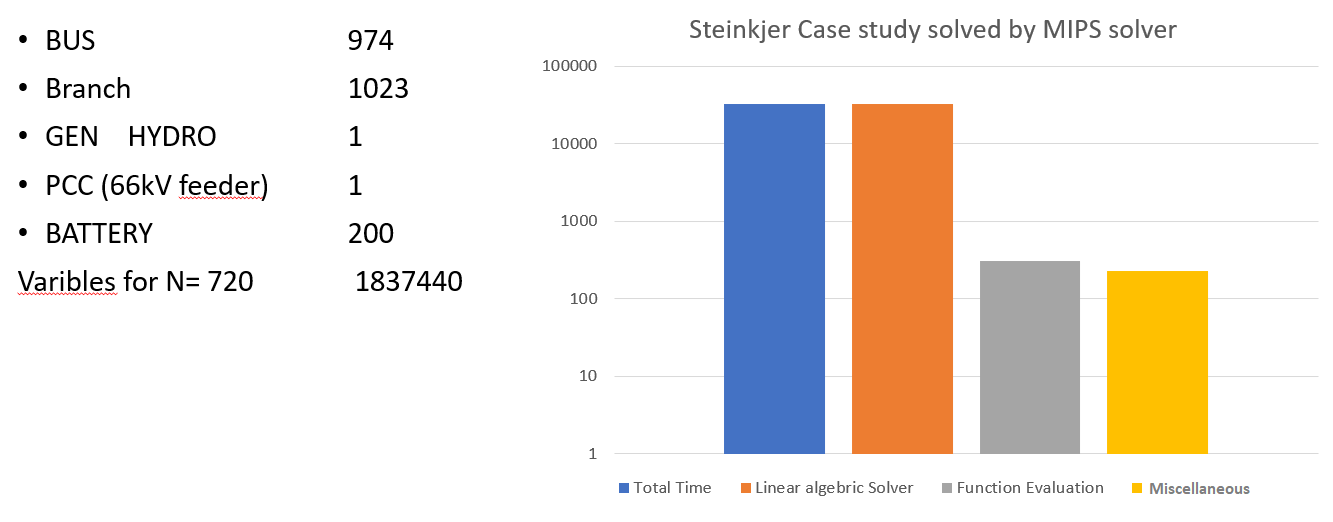
\includegraphics[width=3.5 in , height=1.5 in]{Figures/IPbottleneck.png}
        \end{backgroundblock}}
\end{enumerate}
\end{block}
\end{frame}
%%%%%%%%%%%%%%%%%%%%
%%%%%%%%%%%%%%%5 
%%%%%%%%%%%%%%%%%%%%
%%%%%%%%%%%%%%%5
\begin{frame}[plain]
\begin{tikzpicture}[overlay, remember picture]
\node[anchor=center] at (current page.center) {
\begin{beamercolorbox}[center]{title}
     Phase IV:\\\textbf{Speed-up}
  \end{beamercolorbox}};
\end{tikzpicture}

\end{frame}
%%%%%%%%%%%%%%%%%%%%%%%%%%%%%%%%%%%
%%%%%%%%%%%%%%%%%%%%%%%%%%%%%%%%%
%%%%%%%%%%%%%%%%%%%%%%%%%%%%%%%%%
%%%%%%%%%%%%%%%%%%%%%%%%%%%%%%%%%%%
%%%%%%%%%%%%%%%%%%%%%%%%%%%%%%%%%%%%
%%%%%%%%%%%%%%%%%%%%%%%%%%%%%%%%%%%
%%%%%%%%%%%%%%%%%%%%%%%%%%%%%%%%%
\section{Speedup}
\subsection{Sparsity}
\begin{frame}
\begin{figure}[!htbp]
\centering
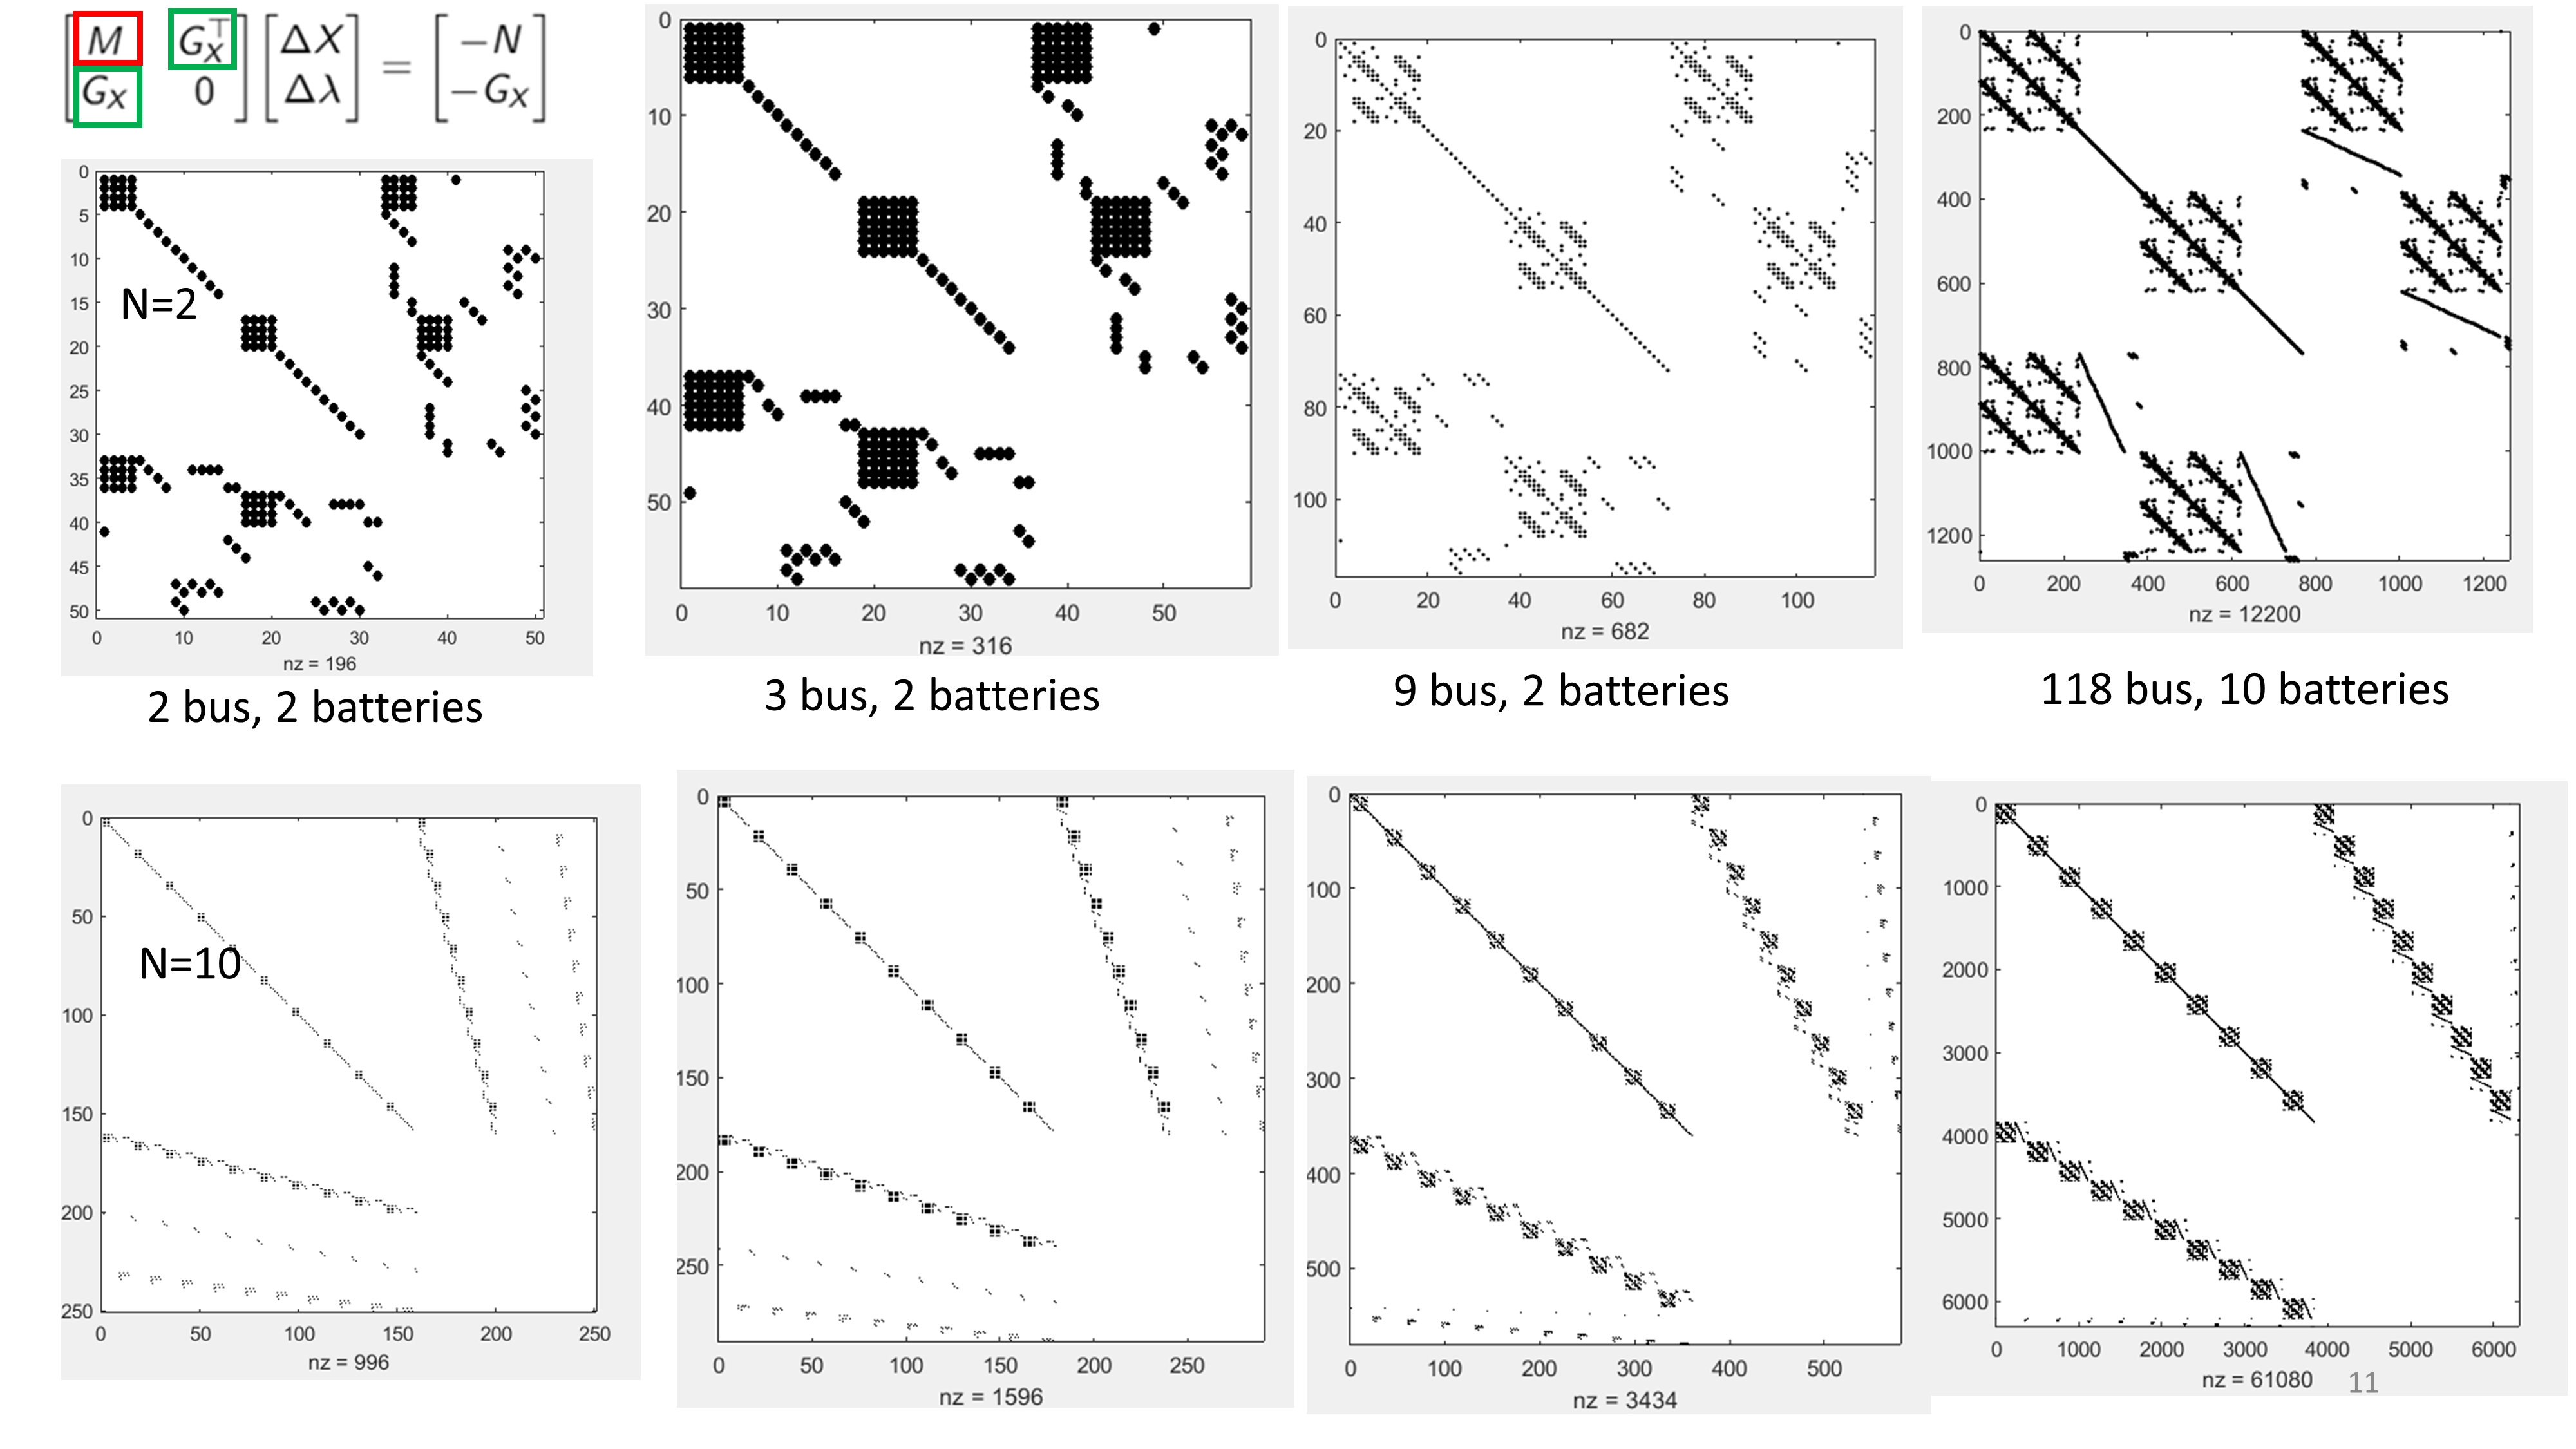
\includegraphics[width=4.1 in , height=2.8 in]{Figures/Sparsity.png}
\caption{Sparse stracture of the Newton-Raphson Jacobian}
\label{sparsity}
\end{figure}
\end{frame}

%%%%%%%%%%%%%%%%%%%%%%%%%%%%%%%%%
%%%%%%%%%%%%%%%%%%%%%%%%%%%%%%%%%%%
%%%%%%%%%%%%%%%%%%%%%%%%%%%%%%%%%%%%
%%%%%%%%%%%%%%%%%%%%%%%%%%%%%%%%%%%
\begin{frame}{Connectivity Matrices}
\begin{center}
\begin{tabular}{|l l|}
\hline
{\tiny a term in pf equation:} & ${\begin{bmatrix} \mathbf{C}_g \end{bmatrix} \ \mkern-10mu}_{n_b \times n_g} {\begin{bmatrix}\mathbf{P}_g \end{bmatrix} \ \mkern-10mu}_{n_g \times 1} $\\
\hline
 \cellcolor{Gray}example: &  \cellcolor{Gray}$ {\textcolor{red}{{\begin{colorbmatrix}
    0&  0 &0 & 0 & 0 \\
    0&1 & 0 &0 &0\\
0 &0 &0 &0&0\\
    1&0 & 0 &0 &0\\
0 &0 &0 &0&0\\
0 &0 &1 &0&0\\
0 &0 &0 &0&0\\
0 &0 &0 &0&0\\
0 &0 &0 &1&0\\
0 &0 &0 &0&1
\end{colorbmatrix} \ \mkern-10mu}_{n_b \times n_g}}}
{\begin{colorbmatrix}
    \mathbf{P}_{g_1} \\
   \mathbf{P}_{g_2}\\ 
\mathbf{P}_{g_3}\\
 \mathbf{P}_{g_4}\\ 
\mathbf{P}_{g_5}\\
\end{colorbmatrix} \ \mkern-10mu}_{n_g \times 1}=
{\begin{colorbmatrix}
0\\
     \mathbf{P}_{g_2} \\
0\\
   \mathbf{P}_{g_1}\\ 
0\\
\mathbf{P}_{g_3}\\
0\\
0\\
 \mathbf{P}_{g_4}\\ 
\mathbf{P}_{g_5}\\
\end{colorbmatrix} \ \mkern-10mu}_{n_b \times 1}$ \\
\hline
\end{tabular}
\end{center}
\end{frame}
%
%%%%%%%%%%%%%%%%%%%%
%%%%%%%%%%%%%%%5
%%%%%%%%%%%%%%%%%%%%
%%%%%%%%%%%%%%%5

\section{Speed-up the solution proposal}
\subsection{Reordering}
\begin{frame}
\begin{figure}[!htbp]
\centering
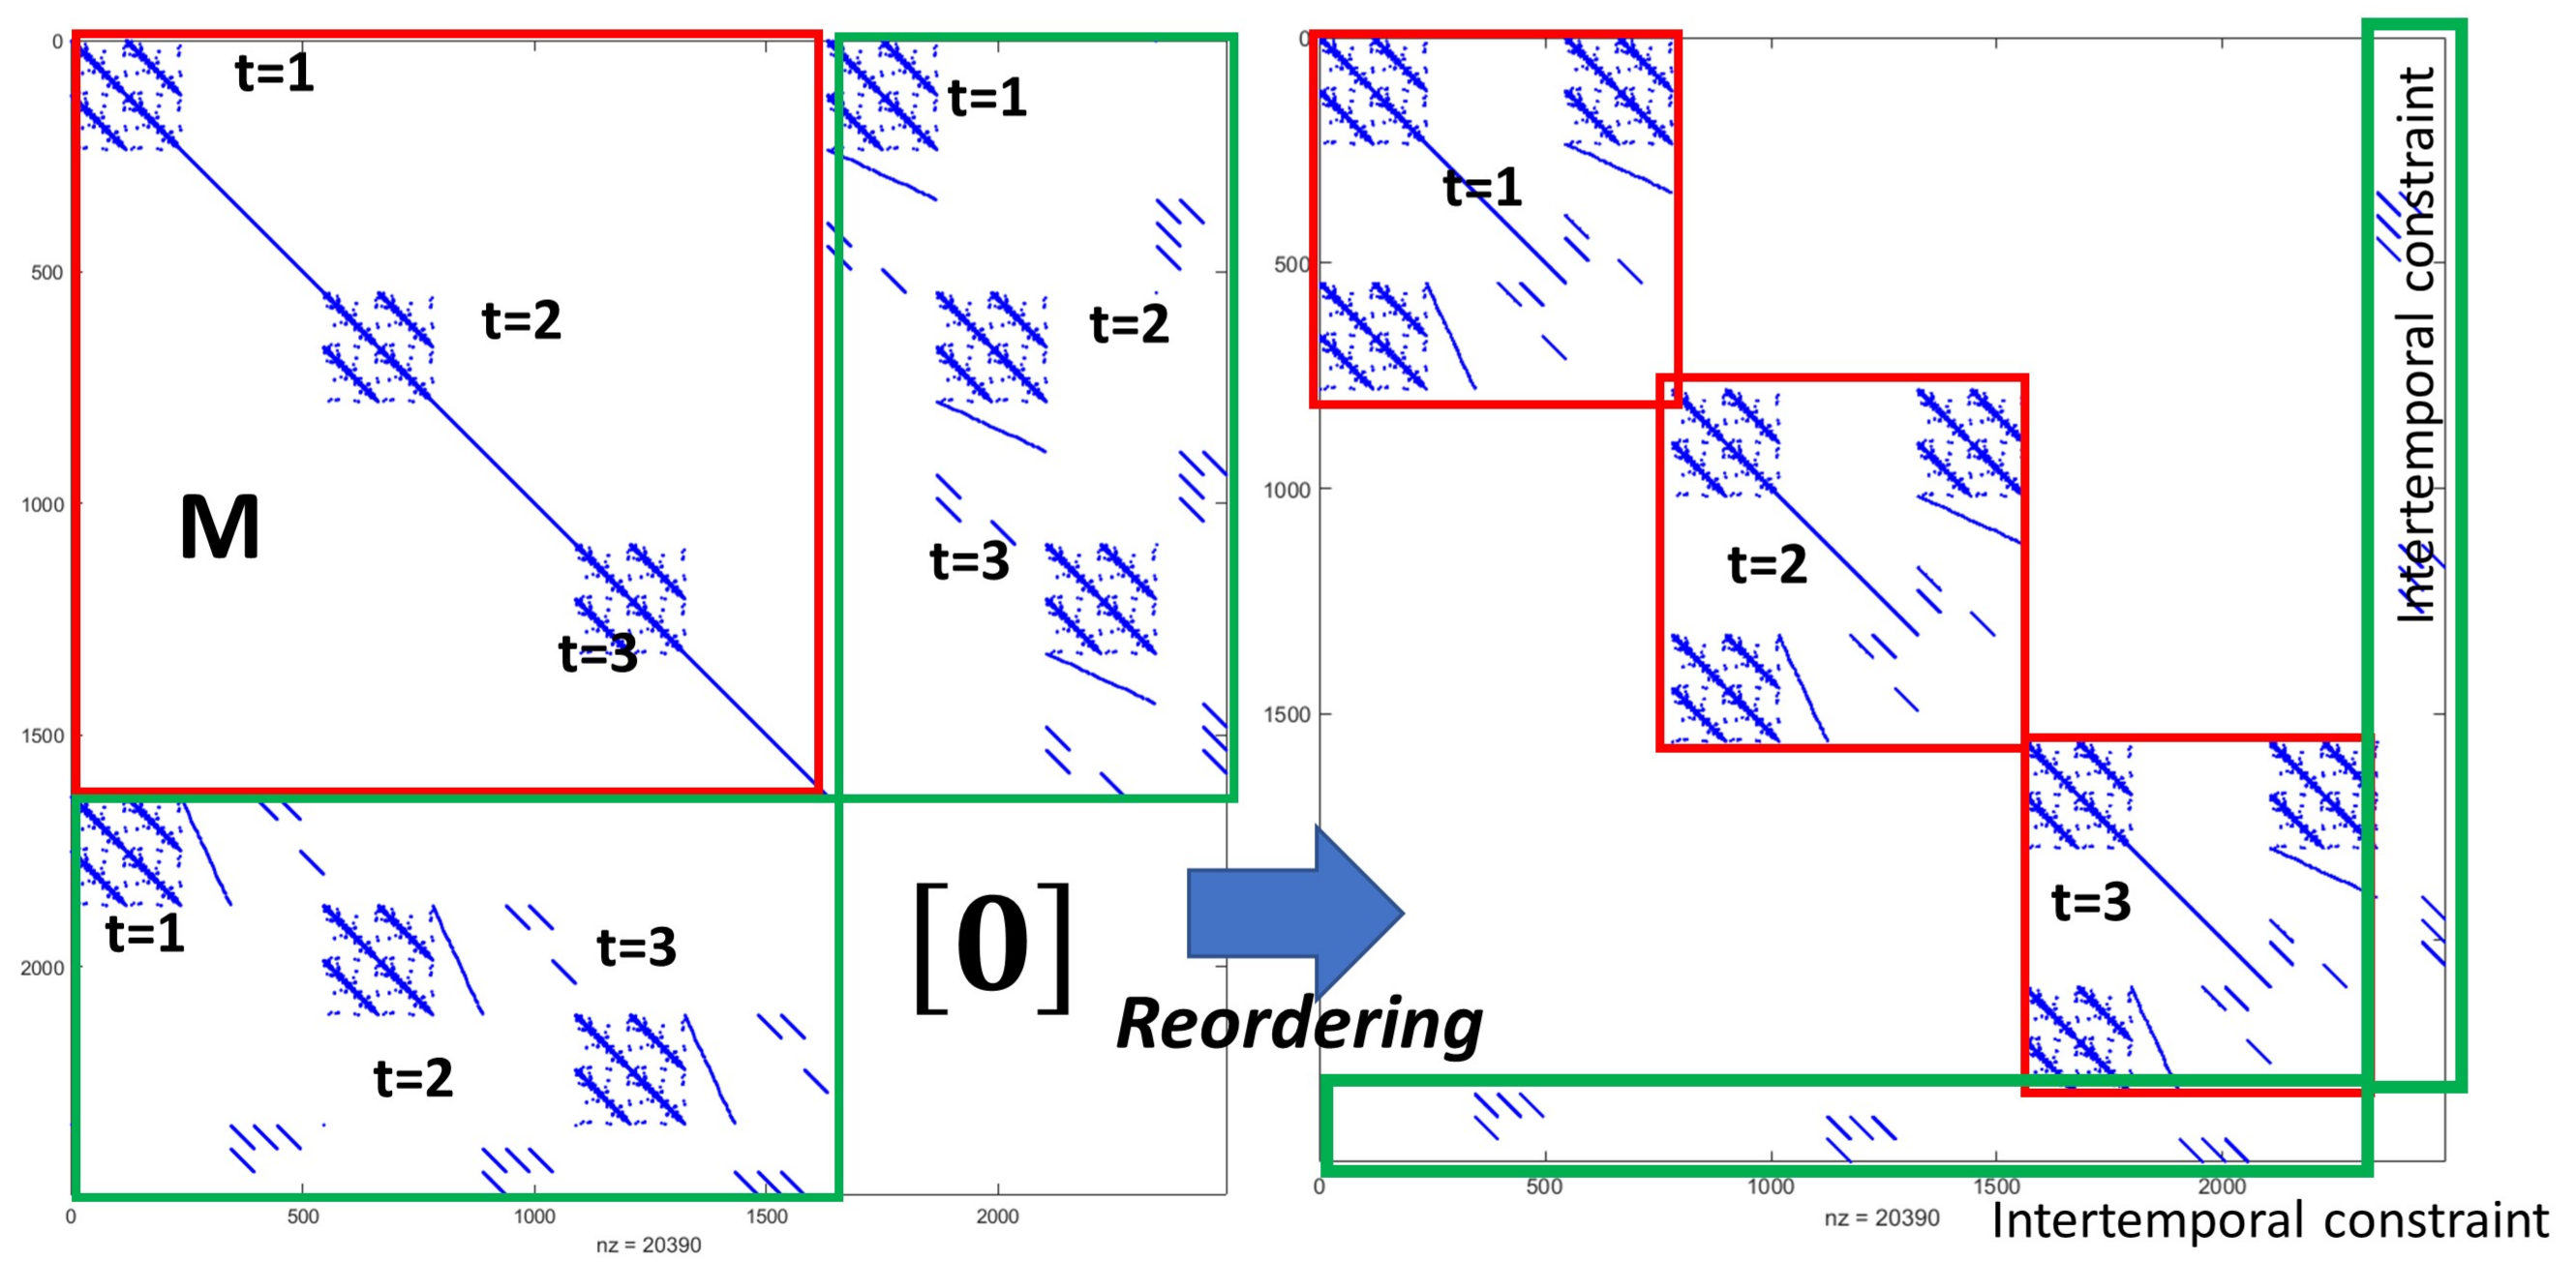
\includegraphics[width=3.4 in , height=1.7 in]{Figures/reorder.png}
% where an .eps filename suffix will be assumed under latex,
% and a .pdf suffix will be assumed for pdflatex; or what has been declared
% via \DeclareGraphicsExtensions.
\caption{Structure of Jacobian of the Newton-Raphson's algorithm before and after reordering.}
\label{fig:1}\vspace*{-0.4cm}
\end{figure}
\begin{alertblock}{Jacobian of Newton-Raphson}
\centering
{\tiny
${\textcolor{red}{\begin{colorbmatrix}
    \mathbf{M}&  \mathbf{G}_{\mathbf{X}}^\top\\
    \mathbf{G}_{\mathbf{X}} & 0\\
\end{colorbmatrix}}}
{\begin{colorbmatrix}
    \Delta \mathbf{X}\\
   \Delta\boldsymbol{\lambda}
\end{colorbmatrix}}=
{\begin{colorbmatrix}
    -\mathbf{N}\\
   -\mathbf{G}(\mathbf{X})
\end{colorbmatrix}} $\\
The solution is published in Papers I and II of this thesis.}
\end{alertblock}
 \end{frame}
%%%%%%%%%%%%%%%%%%%%%%%%%%%%%%%%%
%%%%%%%%%%%%%%%%%%%%%%%%%%%%%%%%%%%
%%%%%%%%%%%%%%%%%%%%%%%%%%%%%%%%%%%%
%%%%%%%%%%%%%%%%%%%%%%%%%%%%%%%%%%%
%%%%%%%%%%%%%%%%%%%%%%%%%%%%%%%%%
%%%%%%%%%%%%%%%%%%%%%%%%%%%%%%%%%
%%%%%%%%%%%%%%%%%%%%%%%%%%%%%%%%%%%
%%%%%%%%%%%%%%%%%%%%%%%%%%%%%%%%%%%%
%%%%%%%%%%%%%%%%%%%%%%%%%%%%%%%%%%%
%%%%%%%%%%%%%%%%%%%%%%%%%%%%%%%%%
\section{Results}
\subsection{Schur-Complement}
\begin{frame}
\begin{figure}[!htbp]
\centering
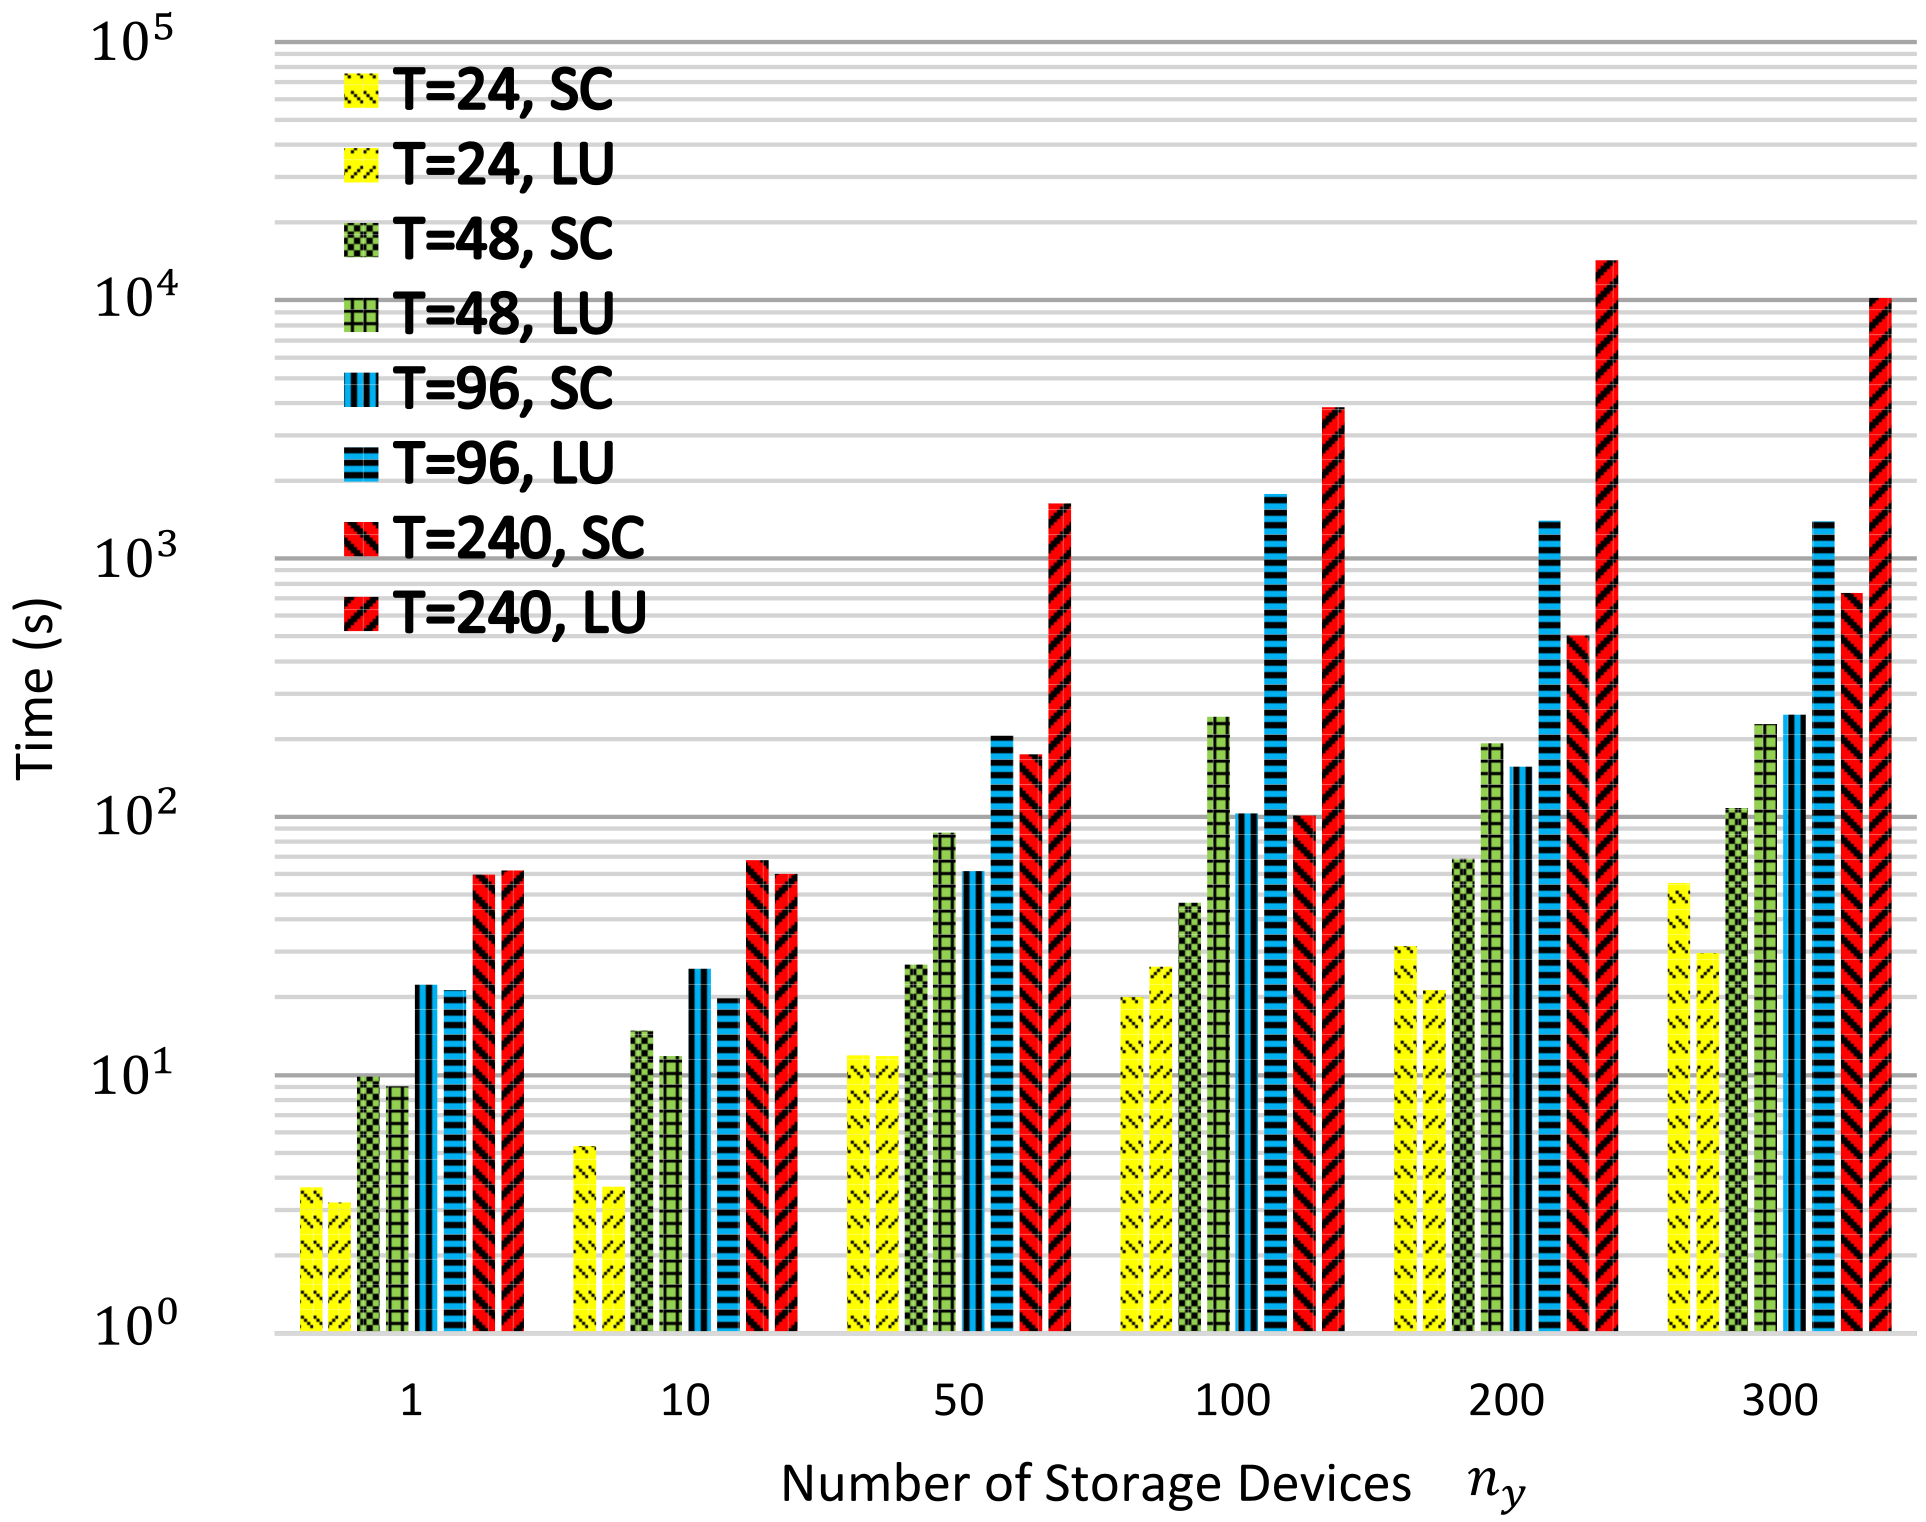
\includegraphics[width=3.0 in , height=2.5 in]{Figures/SCLU118Bus.png}
\caption{Total time ($\mathrm{TotalTime= No_{\cdot} of \ Iter_{\cdot} \times TimePerIter}$) for solution of the linear KKT systems, Case: IEEE 118.}
\label{118bus}
\end{figure}
\end{frame}

%%%%%%%%%%%%%%%%%%%%%%%%%%%%%%%%%
%%%%%%%%%%%%%%%%%%%%%%%%%%%%%%%%%%%
%%%%%%%%%%%%%%%%%%%%%%%%%%%%%%%%%%%%
%%%%%%%%%%%%%%%%%%%%%%%%%%%%%%%%%%%
%%%%%%%%%%%%%%%%%%%%%%%%%%%%%%%%%

\begin{frame}{Analytical Derivatives}
\vskip -0.6cm
\begin{table}
\tiny
\begin{center}
 \caption{Total time ($\mathrm{TotalTime= No_{\cdot} of \ Iter_{\cdot} \times TimePerIter}$) elapsed to calculate: 1) Analytical (hand-coded) derivatives, and 2) Numerical derivatives }
\label{tab:numericVSanalytic}
\begin{threeparttable}
\begin{tabularx}{\textwidth}{m s s s s c s s s c m }
\toprule
&&&&   \multicolumn{3}{c}{Analytical}&&\multicolumn{3}{c}{Numerical} \\
\cmidrule{5-7}  \cmidrule{9-11}
Case     & $T$&$n_y$ &iter & ${F}_\mathbf{X}$(s)&$\mathbf{G}_\mathbf{X}$+ $\mathbf{H}_\mathbf{X}$(s)&$\boldsymbol{\mathcal{L}}_{\mathbf{X}\mathbf{X}}^{\gamma}$(s)& &${F}_\mathbf{X}$(s)&$\mathbf{G}_\mathbf{X}$+ $\mathbf{H}_\mathbf{X}$(s)&$\boldsymbol{\mathcal{L}}_{\mathbf{X}\mathbf{X}}^{\gamma}$(s) \\
\midrule
Case9     &2 &5&13& 0.03 & 0.13 & 0.14 & &0.43 & 0.98 &140.07\\
Case9     &10&5&23& 0.08  & 0.36 & 0.37 & &11.32 & 30.62  & 22815.29\\
IEEE30    &2&5&12 & 0.04 & 0.25 & 0.18     &   & 1.01  & 2.16  & 682.70\\
IEEE30    &10&5&16& 0.05 & 0.24 & 0.25 && 16.73 & 49.12  & 79712.78\\
IEEE118   &2&5&22 & 0.04 & 0.19 & 0.20   & &7.41 & 18.07 & 24557.09\\
IEEE118   &10&5&37&  0.09 & 0.62 & 0.82   & & 158.21\tnote{1}  & 572.09\tnote{1} & 4599735\tnote{1} \\
\begin{tabular}[l]{@{}l@{}}Pegase\\1354  \end{tabular} &2 &5&23& 0.05 & 0.61 & 0.78    & &85.54\tnote{1}  & 496.18\tnote{1} & 7185888\tnote{1}  \\
\begin{tabular}[l]{@{}l@{}}Pegase \\1354  \end{tabular}&10&5&33& 0.10 & 3.77 & 5.15  & & 588.06\tnote{1}  & 3530\tnote{1} & 51550941\tnote{1}  \\
\bottomrule
\end{tabularx}
\begin{tablenotes}
\item[1] {Estimated total time: The time elapsed for one iteration multiplied to the iteration that would take to converge}
\end{tablenotes}
\end{threeparttable}
\end{center}
\end{table}
\begin{alertblock}{Test Cases}
Test cases of Case9, IEEE30, IEEE118, and PEGASE1354 are part of open source MATPOWER library.
\end{alertblock}
\end{frame}

%%%%%%%%%%%%%%%%%%%%%%%%%%%%%%%%%
%%%%%%%%%%%%%%%%%%%%%%%%%%%%%%%%%%%
%%%%%%%%%%%%%%%%%%%%%%%%%%%%%%%%%%%%
%%%%%%%%%%%%%%%%%%%%%%%%%%%%%%%%%%%
%%%%%%%%%%%%%%%%%%%%%%%%%%%%%%%%%
%%%%%%%%%%%%%%%%%%%%%%%%%%%%%%%%%%%%%%%%%%
%%%%%%%%%%%%%%%%%%%%%%%%%%%%%%%%%%%%%%%%%%
%%%%%%%%%%%%%%%%%%%%%%%%%%%%%%%%%%%%%%%%%%
%%%%%%%%%%%%%%%%%%%%%%%%%%%%%%%%%%%%%%%%%%


\begin{frame}[plain]
\begin{tikzpicture}[overlay, remember picture]
\node[anchor=center] at (current page.center) {
\begin{beamercolorbox}[center]{title}
     Phase V:\\\textbf{Future Works}
  \end{beamercolorbox}};
\end{tikzpicture}

\end{frame}

%%%%%%%%%%%%%%%%%%%%%%%%%%%%%%%%% 
%%%%%%%%%%%%%%%%%%%%%%%%%%%%%%%%%%% 
%%%%%%%%%%%%%%%%%%%%%%%%%%%%%%%%%%%% 
%%%%%%%%%%%%%%%%%%%%%%%%%%%%%%%%%%% 
%

\begin{frame}
\centering
Thank you for your attention!\\
		\vskip 0.8cm

\centering

\includegraphics[scale=0.2]{ntnulogo_eng.png}
\end{frame} 

\end{document}


